\documentclass{article}


\usepackage{arxiv}
\usepackage{natbib}
\usepackage[utf8]{inputenc} % allow utf-8 input
\usepackage[T1]{fontenc}    % use 8-bit T1 fonts
\usepackage[colorlinks=true, citecolor = blue]{hyperref}      % hyperlinks
\usepackage{url}            % simple URL typesetting
\usepackage{booktabs}       % professional-quality tables
\usepackage{amsfonts}       % blackboard math symbols
\usepackage{nicefrac}       % compact symbols for 1/2, etc.
\usepackage{microtype}      % microtypography
\usepackage{graphicx, subfigure}
\usepackage{lipsum}
\usepackage{amsmath}
\usepackage{amsthm}
\usepackage{amssymb}
\usepackage{import}
\usepackage{enumitem}
\usepackage{csquotes}
\usepackage{todonotes}
\usepackage{xfrac}


%%% ============================================================================
%%% Theorems.
%%% ============================================================================
\theoremstyle{plain}
\newtheorem{thm}{\protect\theoremname}
\theoremstyle{plain}
\newtheorem{lem}{\protect\lemmaname}
\theoremstyle{definition}
\newtheorem{defn}[thm]{\protect\definitionname}
\theoremstyle{remark}
\newtheorem{rem}[thm]{\protect\remarkname}
\theoremstyle{definition}
\newtheorem{example}[thm]{\protect\examplename}
\theoremstyle{plain}
\newtheorem{cor}[thm]{\protect\corollaryname}
\theoremstyle{plain}
\newtheorem{prop}[thm]{\protect\propositionname}
\theoremstyle{definition}
\newtheorem{xca}[thm]{\protect\exercisename}
\ifx\proof\undefined
\newenvironment{proof}[1][\protect\proofname]{\par
	\normalfont\topsep6\p@\@plus6\p@\relax
	\trivlist
	\itemindent\parindent
	\item[\hskip\labelsep\scshape #1]\ignorespaces
}{%
	\endtrivlist\@endpefalse
}
\providecommand{\proofname}{Proof}
\fi

\providecommand{\corollaryname}{Corollary}
\providecommand{\definitionname}{Definition}
\providecommand{\propositionname}{Proposition}
\providecommand{\examplename}{Example}
\providecommand{\exercisename}{Exercise}
\providecommand{\remarkname}{Remark}
\providecommand{\theoremname}{Theorem}
\providecommand{\lemmaname}{Lemma}

%%% ============================================================================
%%% Macros.
%%% ============================================================================
\DeclareMathOperator{\tr}{tr}
\DeclareMathOperator{\Tr}{Tr}
\DeclareMathOperator{\Var}{Var}
\DeclareMathOperator{\argmin}{argmin}
\DeclareMathOperator{\Cor}{Cor}
\DeclareMathOperator{\Cov}{Cov}
\DeclareMathOperator{\diag}{diag} 
\DeclareMathOperator{\MSE}{\textsc{MSE}} 

\DeclareMathOperator{\argmax}{argmax}
\newcommand{\geomean}{NA}

\title{Please avoid the standardized alpha}

\author{
  Jonas Moss \\
  Department of Mathematics, University of Oslo\\
  PB 1053, Blindern, NO-0316, Oslo, Norway \\
  \it{jonasmgj@math.uio.no}
}

\begin{document}
\maketitle

\begin{abstract}
I argue coefficient alpha should always be preferred over the standardized alpha. For the coefficient alpha is often consistent when the standardized alpha fails to be, but the opposite is rarely the case. Moreover, assuming normality, coefficient alpha and the standardized alpha have the same asymptotic efficiency under the parallel model, the only case when both are consistent. Since coefficient alpha is the maximum likelihood estimator under the normal parallel model, the only reason to prefer the standardized coefficient would be if it had superior small-sample performance. But a small simulation study shows the two alphas perform equally well under small samples.
\end{abstract}

% keywords can be removed
\keywords{reliability \and coefficient alpha \and cronbach's alpha}

\section{Introduction}
The reliability coefficient is the squared correlation between a latent variable $Z$ and its predictor $\hat{Z}$ \citep[][p. 61]{Lord1968-ax}. Just as the squared correlation between two variables $X$ and $Y$ quantifies the degree of linear relationship between them, with $0$ being no linear relationship and $1$ a perfect linear relationship, the reliability coefficient quantifies how well the noise $\hat{Z}$ works as a predictor of $Z$.

In unidimensional psychometric scales with $k$ test items the most popular predictor $\hat{Z}$ is the sum of the test items, $\hat{Z}=X_1 + \cdots + X_k$. This predictor is often called the sum score \citep{McNeish2019-ea}, and the associated reliability is the congeneric reliability \citep{Cho2016-bs}. The sample coefficient alpha is the most popular estimator of the congeneric reliability, and so it has been for a long time \citep{McNeish2018-vu}. A close cousin of coefficient alpha is the standardized coefficient alpha, or standardized alpha for short. The difference between these two alphas is simple to state: To calculate coefficient alpha you use the sample covariance matrix, to calculate the standardized alpha you use the sample correlation matrix.



I argue you should avoid standardized alpha in all circumstances. I make my case with two arguments:

\begin{enumerate}[label=\arabic*.]
\item I compare standardized alpha to the coefficient alpha as estimators of the congeneric reliability. Standardized alpha is reasonable estimator of the congeneric only under the parallel model, but I argue you should prefer coefficient alpha even if you have good reasons to believe in the parallel model. While the population values of standardized alpha and coefficient alpha both equal the congeneric reliability under the parallel model, coefficient alpha equals the congeneric reliability under the more general $\tau$-equivalent model. But standardized alpha will be greater than the congeneric reliability under the $\tau$-equivalent model. Moreover, sample coefficient alpha is the maximum likelihood estimator of the congeneric reliability under the normal parallel model, which provides a decent heuristic argument in favor of coefficient alpha. Finally, provided the observed variables have finite fourth moments, sample coefficient alpha and sample standardized alpha have the same asymptotic variances. 

\item A common stance on sample standardized alpha is to use it only with standardized test scores. In this case, sample standardized alpha is best understood as an estimator of the standardized reliability, i.e. the squared correlation between $Z$ and $\hat{Z}$ when $\hat{Z}$ is the sum of standardized test items. However, the standardized alpha equals the standardized reliability only under restrictive and unrealistic conditions. If you are willing to go for another kind reliability than the congeneric reliability, I would suggest you consider coefficient $H$ instead, which corresponds to the optimal linear predictor $\hat{Z}$. If coefficient $H$ is too hard to swallow, I propose to standardize with the the residual errors and use the new $\omega_\sigma$ reliability.
\end{enumerate}

In the section \ref{sec:coefficienta alpha} I introduce coefficient alpha, the standardized alpha, and the notion of reliability. I make an effort to be mathematically precise here, and reiterate several known properties about the alphas in a Proposition \ref{prop:Reliabilities.}. I devote section \ref{sec:arument 1} to fleshing out argument 1 and section \ref{sec:argument 2} to argument 2. I end with some brief remarks in section \ref{sec:remarks}.
\section{Coefficient alpha and standardized alpha}
\label{sec:coefficienta alpha}

Let $X$ be random variable in $\mathbb{R}^{k}$ with finite variance.
Let $\Sigma=\Cov X$ be the covariance matrix of $X$ and $\Phi=\Cor X$
be the correlation matrix of $X$. Let $\mathbf{i}=\left(1,1,\ldots,1\right)$ by a vector of ones of the appropriate size and $\tr$ be the trace operator.
The population coefficient alpha \citep[][eq. 2]{cronbach1951coefficient} is
\begin{equation}
\alpha =  \frac{k}{k-1}\left(1-\frac{\tr\Sigma}{\mathbf{i}^{T}\Sigma\mathbf{i}}\right)\label{eq:Coefficient alpha}
\end{equation}
and the population standardized alpha \citep[][eq. 2]{Falk2011-ae} is
\begin{equation}
\alpha_s=\frac{k}{k-1}\left(1-\frac{k}{\mathbf{i}^{T}\Phi\mathbf{i}}\right)\label{eq:standardized alpha}
\end{equation}
We care about these alphas since they sometimes coincide with the reliability coefficient under the congeneric model, a special case of the linear one-factor model. Let $Z$ be a mean zero latent variable with unit variance and $\epsilon=\left(\epsilon_{1},\epsilon_{2},\ldots,\epsilon_{k}\right)$
be a mean zero vector of uncorrelated errors with unit variance. In addition, assume $Z$ and $\epsilon$ are uncorrelated. Define the congeneric model
\begin{equation}
X=\alpha + \lambda Z+\Psi^{1/2}\epsilon\label{eq:one-factor model}
\end{equation}
where $\lambda$ is a vector of loadings, $\alpha$ is a mean vector, and $\Psi^{1/2}$ is a diagonal matrix with positive diagonal elements $\sigma_i$. Since $\Psi^{1/2}$ is diagonal the errors $\Psi^{1/2}\epsilon$ are uncorrelated. When $\Psi^{1/2}$ is allowed to be any positive definite matrix, the model \eqref{eq:one-factor model} is a one-factor model. We made no parametric assumptions about either $Z$ or $\epsilon$, and right now they can have any distribution whatsoever. Since $\alpha,\lambda,\Psi$ are parameters of the model, we are dealing with a semi-parametric model.

Let $\hat{Z}$ be a linear predictor of $Z$ based on $X$, that
is there are some real weights $w_{i},i=1,\ldots,k$ such that
\begin{equation}
\label{eq:Linear predictor}
\hat{Z} =  \sum_{i=1}^{k}w_{i}X_i =  \sum_{i=1}^{k}w_{i}\left(\lambda Z+\sigma_{i}\epsilon\right).\nonumber 
\end{equation}
The reliability of $\hat{Z}$ as a predictor of $Z$ is $\omega =\Cor^{2}(\hat{Z},Z)$. Since $\hat{Z}$ is determined by its weights $w_i$, I will sometimes talk about the reliability with weights $w_i$.

The purpose of the reliability coefficient is to tell us how well a linear predictor $\hat{Z}$ predicts $Z$. In this sense it is analogous to $R^2$ from linear regression. The following proposition makes this claim precise. In this proposition, and the rest of the paper, I will use the notation $\overline{x}$ to denote the mean of the vector $x$.

\begin{prop}
\label{prop:reliability motivation}Assume the congeneric model \eqref{eq:one-factor model}. Let $\hat{Z}=\sum_{i=1}^{k}w_{i}X$
for some weights $w_{i},i=1,\ldots,k$. Then the reliability equals
\begin{eqnarray}
\omega & = & \frac{(w^{T}\lambda)^{2}}{(w^{T}\lambda)^{2}+w^{T}\Psi w}\label{eq:linear reliabiltiy}\\
 & = & 1- \MSE (w_{0}\hat{Z})\nonumber 
\end{eqnarray}
where $\MSE (w_{0}\hat{Z})=E[(Z-w_{0}\hat{Z})^{2}]$ is the
mean squared error and $w_{0}=\overline{w\lambda}/(k\overline{w\lambda}^{2}+\overline{w^{2}\sigma^{2}})$ is the constant minimizing the mean squared error.
\end{prop}
\begin{proof}
See the appendix, page \pageref{proof:reliability motivation} for a proof.
\end{proof}

Equation \eqref{eq:linear reliabiltiy} is the definition \citet[][p. 112]{Joreskog1971-nn} gave of the composite reliability of under the congeneric model \eqref{eq:one-factor model}. The role of $w_0$ in Proposition \ref{prop:reliability motivation} is to make sure $\hat{Z}$ predicts $Z$ on he right scale, and in this paper the scale of $Z$ is fixed by $\Var Z = 1$. Since $Z$ is latent we would usually not care about this scale, but it is handy to fix it to $1$ since it allows us to compare different predictors of $\hat{Z}$. The formulation $1-\MSE (w_{0}\hat{Z})$ is more concrete than the correlation formulation, as it explicitly references the predictor $w_{0}\hat{Z}$, while the correlation is scale-free and more abstract. The mean squared error definition is amenable to generalizations too, and I will explore one such generalization in future paper. 

A modestly popular choice for $w$ are the weights minimizing the mean squared error (or equivalently, maximizing the reliability $\omega$), known as the Thurstone \citep{thurshronebook} weights. Using these weights lead to coefficient $H$ \citep{hancock2001rethinking}, also known as the maximal reliability \citep{Li1997-yh}, 
\begin{equation}
\label{eq:coefficient_H}
\omega_{H}=\frac{k\overline{\lambda^{2}\sigma^{-2}}}{k\overline{\lambda^{2}\sigma^{-2}}+1},
\end{equation}
where $\overline{\lambda^{2}\sigma^{-2}} = k^{-1}\sum_{i=1}^{k}\lambda_{i}^2/\sigma_i^2$. But by far the most popular choice is give to same weight to each $X_i$, or $w = \mathbf{i}=\left(1,1,\ldots,1\right)$. This leads to the congeneric reliability
\begin{equation}
\omega =\frac{k\overline{\lambda}^{2}/\overline{\sigma^{2}}}{k\overline{\lambda}^{2}/\overline{\sigma^{2}} + 1}\label{eq:Congeneric reliability}
\end{equation}
where $\overline{\lambda}=k^{-1}\sum_{i=1}^{k}\lambda_{i}$ and
$\overline{\sigma^{2}}=k^{-1}\sum_{i=1}^{k}\sigma_{i}^{2}$. Finally, the weights $w_i = \sqrt{\lambda_i^2 + \sigma_i^2}$ yield the standardized reliability, which is closely related to standardized alpha.
\begin{equation}
\omega_s=\frac{k\overline{\lambda(\lambda^{2}+\sigma^{2})^{-1/2}}^{2}/\overline{\sigma^{2}(\lambda^{2}+\sigma^{2})^{-1}}}{k\overline{\lambda(\lambda^{2}+\sigma^{2})^{-1/2}}^{2}/\overline{\sigma^{2}(\lambda^{2}+\sigma^{2})^{-1}}+1}.\label{eq:Standardized reliability}
\end{equation}
It is time to relate the reliabilities to the alpha coefficients.
Define the generalization of the coefficient alpha and the standardized
alpha, the \emph{weighted alpha},
\begin{equation}
\alpha_{w}=\frac{k}{k-1}\left(1-\frac{w^{T}\diag\Sigma w}{w^{T}\Sigma w}\right)\label{eq:weighted alpha}
\end{equation}
The ordinary coefficient alpha \eqref{eq:Coefficient alpha} has weights $w=\mathbf{i}$
while the standardized alpha \eqref{eq:standardized alpha} has weights $w_{i}=\sqrt{\lambda_{i}^{2}+\sigma_{i}^{2}}$. Coefficient alpha and standardized alpha are the most interesting cases of the weighted alpha as you can calculate them using only the covariance matrix $\Sigma = \Cov X$, but the definition makes sense for any weight $w$. The following Proposition summarizes the basic relationship
between the reliability $\omega_{w}$ and the weighted $\alpha_{w}$. To state it, we will need
the notion of a \emph{$\tau$-equivalent model} \citep[][section 2.13]{Lord1968-ax}. A congeneric model \eqref{eq:one-factor model} is $\tau$-equivalent if $\lambda_{i}=\lambda_{j}$ for all $i,j$. That is, all unstandardized
factor loadings are equal.
\begin{prop}
\label{prop:weighted alpha}. Let $w$ be a vector of weights and
assume $X$ follows the congeneric model \eqref{eq:one-factor model}. Then $\alpha_{w}\leq\omega_{w}$
with equality if and only if $wX$ is $\tau$-equivalent, i.e. $\lambda_{i}=\lambda_{j}$
for all $i,j$.
\end{prop}

\begin{proof}
The result for coefficient alpha is classical, see \citep[][pp. 87 -- 89]{Lord1968-ax}. See the appendix page \pageref{proof:weighted alpha}
for a proof.
\end{proof}

When $w_{i}=\sqrt{\lambda_{i}^{2}+\sigma_{i}^{2}}$, $wX$ is $\tau$-equivalent if only if the standardized factor loadings are equal, and Proposition \ref{prop:weighted alpha} tells us $\alpha_s = \omega_s$ in this case. But $\alpha =\alpha_s$ are equal when both $X$ and $wX$ are $\tau$-equivalent, which happens if and only if both $\lambda_{i}=\lambda_{j}$
and $\sigma_{i}=\sigma_{j}$. A congeneric model satisfying this strong property is a \emph{parallel model} \citep[][section 2.13]{Lord1968-ax}. 

The next propositions explores the relationship between coefficient alpha, the standardized alpha, and the congeneric reliability coefficient.

\begin{prop}
\label{prop:Reliabilities.}Assume the congeneric model \eqref{eq:one-factor model}. Let $\alpha$ be coefficient alpha \eqref{eq:Coefficient alpha}, $\alpha_{s}$ be the standardized alpha \eqref{eq:standardized alpha}, and  $\omega$ be the congeneric reliability \eqref{eq:Congeneric reliability}. 
\begin{enumerate}[label=(\roman*)]
\item Coefficient alpha equals $$\alpha=\omega-\left(\frac{\overline{\lambda^{2}}-\overline{\lambda}^{2}}{k\overline{\lambda}^{2}+\overline{\sigma^{2}}}\right),$$
and $\alpha\leq\omega$ with equality
if and only if $\lambda_{i}=\lambda_{j}$ for all $i,j$.
\item Assume $\lambda_{i}=\lambda_{j}$ and for all $i,j$. Then $\alpha_s \geq \alpha = \omega(X)$, with equality if and only if $\sigma_{i}^{2}=\sigma_{j}^{2}$ for all $i,j$ or $\lambda_i = 0$ for all $i$.
\item If $k=2$, $\alpha_s\geq\alpha$, with equality if and only if $\lambda_{1}^{2}+\sigma_{1}^{2}=\lambda_{2}^{2}+\sigma_{2}^{2}$ or $\lambda_1 = 0$ or $\lambda_2 = 0$. But if $k>2$, both $\alpha_s>\alpha$
and $\alpha_s<\alpha$ are possible.
\item All of $\alpha_{s}=\omega$, $\alpha_{s}>\omega$ and $\alpha_{s}<\omega$
are possible when $\lambda_{i}\neq\lambda_{j}$ for some $j$.
\end{enumerate}
\end{prop}
\begin{proof}
Most of (i) -- (iv) have been known for a while. See page \pageref{proof:Reliabilities.} of the appendix for a proof.
\end{proof}

If $\lambda_{i}=\lambda_{j}$ for all $i,j$ and $\sigma_{i}=\sigma_{j}$
model \eqref{eq:one-factor model} is called a parallel model \citep[][section 2.13]{Lord1968-ax}. If $\lambda_{i}=\lambda_{j}$
for all $i,j$ it is a $\tau$-equivalent model \citep[][section 2.13]{Lord1968-ax}. The take-messages of Proposition \ref{prop:Reliabilities.} are:

\begin{enumerate}[label=(\alph*)]
\item $\alpha = \omega$ under the $\tau$-equivalent model and,
\item $\alpha_s = \omega$ under the parallel model and,
\item $\alpha \leq \omega(X)$, hence coefficient alpha is a lower bound for the congeneric reliability and,
\item $\alpha_s \geq \alpha = \omega(X)$ under the $\tau$-equivalent model.
\end{enumerate}

Of these, (a) and (b) are the most important, as they give use a way to estimate the congeneric reliability $\omega$ \eqref{eq:Congeneric reliability} using only a simple function of $S$. The intuitive estimate of $\omega$ is the plug-in estimator, which requires us to estimate $\lambda$ and $\sigma$ first. This is usually a more complicated procedure involving Newton-Raphson and so on [[ref]]. Just be aware this advantage of $\alpha_s$ and $\alpha$ is not decisive, as it is easy to estimate $\lambda$ and $\Psi$ these days using for instance the \texttt{R} \citep{Team2013-tt} package \texttt{lavaan} \citep{Rosseel2012-yg}. And estimating $\omega$ this way allows us to forego the unrealistic assumptions of $\tau$-equivalence and parallel test items altogether.

I must emphasize we do not have to assume normality or continuous $X$s to get Proposition \ref{prop:Reliabilities.}. In fact, none of the derivations in Proposition \ref{prop:Reliabilities.} involve the distributions of $Z$ and $\epsilon$. This is contrary to some claims about coefficient alpha in the literature, e.g. \citep[][p.415]{McNeish2018-vu} and \citep[][p.21]{Zumbo2007-ap}. Tankov [[ref]] has lamented this widespread misunderstanding.

While $\alpha_s$ is an upper bound for $\alpha$ when $k = 2$ and under the $\tau$-equivalent model, it does not bound $\alpha$ in either direction otherwise, see Proposition \ref{prop:Reliabilities.} (i - iii). Again, this is contrary to claims in the literature such as that of \citep[][p.348]{Osburn2000-jd} \enquote{When the components of a composite measure are congeneric, standardized alpha will always exceed the true reliability}. See \citet[][p.450]{Falk2011-ae} for a clearly laid out example of $\alpha>\alpha_s$.

Coefficient alpha equals the congeneric reliability if and only if all the factor loadings $\lambda$ are equal, see Proposition \ref{prop:Reliabilities.} (i). But there is no simple necessary and sufficient criterion for $\alpha_s = \omega$: the assumption that all fact merely sufficient. See the proof of Proposition \ref{prop:Reliabilities.} (iv) (page \pageref{proof:Reliabilities.} for a method to generate cases when $\alpha_s = \omega$ but the model is not parallel. Still, these causes are like lucky conincidences. It would be preposterous to assume $\alpha_s = \omega$ for unknown parameter values without assuming the parallel model.

Let us proceed to the sample variants of coefficient alpha and standardized
alpha. Let $S$ be a sample covariance matrix based on
$n$ samples of $X$ and $R$ the corresponding correlation matrix.
The sample coefficient alpha is 
\begin{equation}
\widehat{\alpha}=\frac{k}{k-1}\left(1-\frac{\tr{S}}{\mathbf{i}^{T}S\mathbf{i}}\right)\label{eq:sample coefficient alpha}
\end{equation}
while the sample standardized alpha is
\begin{equation}
\widehat{\alpha}_s=\frac{k}{k-1}\left(1-\frac{k}{\mathbf{i}^{T}R\mathbf{i}}\right)\label{eq:sample standardized alpha}
\end{equation}
The congeneric reliability \eqref{eq:Congeneric reliability} has no
simple sample version, as it depends on estimates of $\lambda$ and
$\sigma^{2}$ which usually do not have closed forms.

The sample coefficient alpha is by far the most popular method to
measure reliability in psychology [[cite]], despite the stringent conditions
that must be satisfied for its population value to be equal to the
true reliability $\omega$ and the questionable choice of weights $w$ \citep{McNeish2019-ea}. This has been lamented by psychometricians such as \citet{McNeish2018-vu} and \citet{Sijtsma2009-hj}. For a spirited defense of sample coefficient alpha see \citep{Raykov2019-yr}.

\section{Argument 1. Standardized alpha as an estimator of the congeneric reliability}
\label{sec:arument 1}

In this section, I will compare sample coefficient alpha \eqref{eq:sample coefficient alpha} to sample standardized alpha \eqref{eq:sample standardized alpha} as estimators of the congeneric reliability \eqref{eq:Congeneric reliability}. From Proposition \ref{prop:Reliabilities.} we know the parallel model is the natural setting to make comparisons, as this is the only case when coefficient alpha and the standardized alpha equals the congeneric reliability.

The parallel model is
\eqref{eq:one-factor model},
\begin{equation}
\label{eq:parallel model}
Y = \alpha + \lambda Z + \sigma\epsilon,
\end{equation}
where $\lambda$ and $\sigma$ are positive scalars and $\epsilon\in\mathbb{R}^k$ and $Z\in\mathbb{R}$ are uncorrelated random variables with unit variance and zero mean. Model \eqref{eq:parallel model} is clearly a special case of \eqref{eq:one-factor model}. Our goal is to estimate the congeneric reliability \eqref{eq:Congeneric reliability}, which for the parallel model equals
\begin{equation}
\label{eq:parallel_omega}
\omega = \frac{k\lambda^2/\sigma^2}{k\lambda^2/\sigma^2 + 1}
\end{equation}
Now we have a model, a parameter, and two competing estimators of that parameter, namely $\widehat{\alpha}$ and $\widehat{\alpha}_s$. But which should we choose? 

Choosing between estimators is a classical statistical problem. Some well-established methods to attack such problems are:

% Let $\rho = \lambda^2/\sqrt{\lambda^2 + \sigma^2}$ be the unique off-diagonal correlation of $\Cor(x)$. 

\begin{enumerate}[label=(\Alph*)]
\item Check the relative asymptotic efficiency of the estimators.
\item Is any of the competing estimators a maximum likelihood estimator, perhaps under some parametric restrictions?
\item Compare finite-sample perfomance of the estimators in terms of for instance mean squared error.
\item Investigate the robustness of the estimators.
\end{enumerate}

In the rest of this section I will argue that coefficient alpha wins (B) and clearly wins (D), standardized alpha might win (C), and (A) is a draw.  

Point (D) about robustness is an easy one, for we have already established that coefficient alpha is more robust than the standardized alpha. For by Proposition \ref{prop:Reliabilities.}, coefficient alpha equals the congeneric reliability under the $\tau$-equivalent model and standardized alpha does not. Thus we can check (D) off our list as a victory for coefficient alpha.

\subsection{Maximum likelihood}
In this section we will work with the parallel model \eqref{eq:parallel model} where $Z$ and $\epsilon$ are independent standard normals. Call this model the normal parallel model.

Coefficient alpha is "usually" the maximum likelihood estimator of $\omega$ in the normal parallel model, see Theorem \ref{thm:ML} for details. Why does this matter? For one thing, maximum likelihood estimators are guaranteed to be efficient under quite weak conditions \citep[][Section 7.3]{Lehmann2004-ke}. But maximum likelihood also has an heuristic justification; maximizing likelihood is an intuitive procedure and is the most popular recipe for making estimators.

\begin{thm}\label{thm:ML}
Assume the parallel model \eqref{eq:parallel model} and that $(Z,\epsilon)$ is multivariate normal. 
\begin{enumerate}[label=(\roman*)]
\item The maximum likelihood estimates of $\lambda^{2}$
and $\sigma^{2}$ are 
\begin{eqnarray*}
\widehat{\lambda^{2}} & = & \begin{cases}
\frac{1}{k-1}\left(\frac{\mathbf{i}^{T}S\mathbf{i}}{k}-\frac{\tr{S}}{k}\right) & \mathbf{i}^{T}S\mathbf{i}\geq\tr{S},\\
0 & \text{\textrm{otherwise}},
\end{cases}\\
\end{eqnarray*}
and
\begin{eqnarray*}
\widehat{\sigma^{2}} & = & \begin{cases}
\frac{1}{k-1}\left(\tr{S}-\frac{\mathbf{i}^{T}S\mathbf{i}}{k}\right) & \mathbf{i}^{T}S\mathbf{i}\geq\tr{S},\\
\frac{\tr{S}}{k} & \textrm{otherwise}.
\end{cases}
\end{eqnarray*}
\item The maximum likelihood estimator of the congeneric reliability
\eqref{eq:Congeneric reliability} equals the sample coefficient alpha
when $\mathbf{i}^{T}S\mathbf{i}\geq\tr{S}$ and $0$ otherwise,
\begin{eqnarray*}
\widehat{\omega} & = & \begin{cases}
\widehat{\alpha}(S) & \mathbf{i}^{T}S\mathbf{i}\geq\tr{S},\\
0 & \text{\textrm{otherwise}}.
\end{cases}
\end{eqnarray*}
\end{enumerate}
\end{thm}
\begin{proof}
See page \pageref{proof:ML} of the appendix for a proof. \citet[][section 3 -- 5]{Kristof1969-ou} worked out the maximum likelihood estimator under the $\tau$-equivalent model, but found no analytic form. \citep[][Exercise 3.9, p. 114]{Muirhead2009-kq} is about the same problem in a different parameterization.
\end{proof}

\subsection{Asymptotic efficiency}
[[fill in: some words about efficiency for the uinitiated; Lehmann as a reference.]]

Efficiency ref: \citep[][Section 4.3]{Lehmann2004-ke}

An estimator $\widehat{\theta}$ efficient if its asymptotic variance is smaller than any other estimator. Maximum likelihood estimators are efficient under weak conditions, hence $\alpha$ is efficient under the normal parallel model by Theorem \ref{thm:ML}.

Asymptotic relative efficiency is possibly the most popular method to compare estimators. Let $\widehat{\theta}_2$ and $\widehat{\theta}_2$ be two estimator converging to a normal distribution at with $n^{1/2}$-rate to the same parameter $\theta$, i.e. 
$n^{1/2}{(\widehat{\theta}_1 - \theta)}$ and $n^{1/2}{(\widehat{\theta}_2 - \theta)}$ both converge to mean-zero normal distributions. The variances of these two distributions do not have to be the same though. Denote the variance of the first distribution $\phi_1^2$ and the variance of the second distribution $\phi_2^2$. Then the asymptotic relative efficiency of $\widehat{\theta_1}$ vs $\widehat{\theta_2}$ is $\phi_2^2/\phi_1^2$.

An estimator $\widehat{\theta}$ efficient if its asymptotic variance is smaller than any other estimator. Maximum likelihood estimators are efficient under weak conditions, hence $\alpha$ is efficient under the normal parallel model by Theorem \ref{thm:ML}.

\begin{thm}
\label{thm:asymptotics}
Assume $X$ has finite variance. 
\begin{enumerate}[label=(\roman*)]
    \item Both sample coefficient alpha and sample standardized alpha converge to their population counterparts with probability $1$. Under the parallel model they are strongly consistent and converge to the congeneric reliability. That is, $\widehat{\alpha}\to\alpha$ and $\widehat{\alpha}_s\to\alpha_s$ with probability $1$ and $\alpha = \alpha_s = \omega$.
    \item Under the parallel model \eqref{eq:parallel model} coefficient alpha and standardized alpha share a normal limit distribution when $Z$ and $\epsilon$ have finite fourth moments, i.e. $\sqrt{n}(\widehat{\alpha} - \alpha) = \sqrt{n}(\widehat{\alpha}_s - \alpha_s)$ both converges to the same normal variable $Z$.
    \item Under the normal parallel model, both $\alpha$ and $\alpha_s$ are efficient. Their common limit is normal with asymptotic variance 
    $$\sigma^{2}\left(\alpha\right)= \sigma^{2}\left(\alpha_{s}\right)=2\frac{k}{k-1}\left(1-\alpha_{s}\right)^{2},$$
    where $\rho$ is the unique correlation of the covariance matrix $\Phi$.
\end{enumerate}
\end{thm}    
\begin{proof}
See page \pageref{proof:asymptotics} of the appendix. The proofs of (ii) and (iii) rely heavily on \citep{Van_Zyl2000-si} and \citep{hayashi2005note}. \citep{Raykov2019-tv} has a proof of (i) and is an introduction to convergence with probability $1$ in the psychometry context.
\end{proof}

Time for some remarks about Theorem \ref{thm:asymptotics}. (i) States that both $\widehat{\alpha}_s$ and $\widehat{\alpha}$ estimate what they should. 

A straightforward consequence of Theorem \ref{thm:ML} is that $\widehat{\alpha}$ is efficient under the normal parallel model, and in this sense (iii) is an extension of said theorem. The shared limit distribution is simple enough to be usable in practice for both estimators. 

Theorem \ref{thm:asymptotics} (ii) is the main argument result of this section. It shows $\alpha_{s}$ and $\widehat{\alpha}$ equally well in the limit no matter what $\lambda$, $\sigma$ and the distributions of $Z$, $\epsilon$ is. We only require that the models have finite fourth moments.

\subsection{A small simulation}
There is no reason to choose standardized alpha over coefficient alpha from an efficiency standpoint. But it might still be the case
that the standardized alpha outperforms coefficient alpha
in small samples. I have devoted this section to a small simulation
study comparing the mean squared error of the estimators under
the parallel model. Since the coefficient alpha is the maximum likelihood
estimator for the normal parallel model there is some heuristic reason
to believe it will perform better than the standardized estimator
in this context. Instead of normal errors I will use three non-normal
errors distributions:

\begin{enumerate}
\item Scaled $t$-distribution with $5$ degrees of freedom. The $t$-distribution
has heavier tails than the normal distribution but is symmetric and nearly bell-shaped. 
\begin{figure}
	\centering     %%% not \center
	\subfigure[Beta distribution]{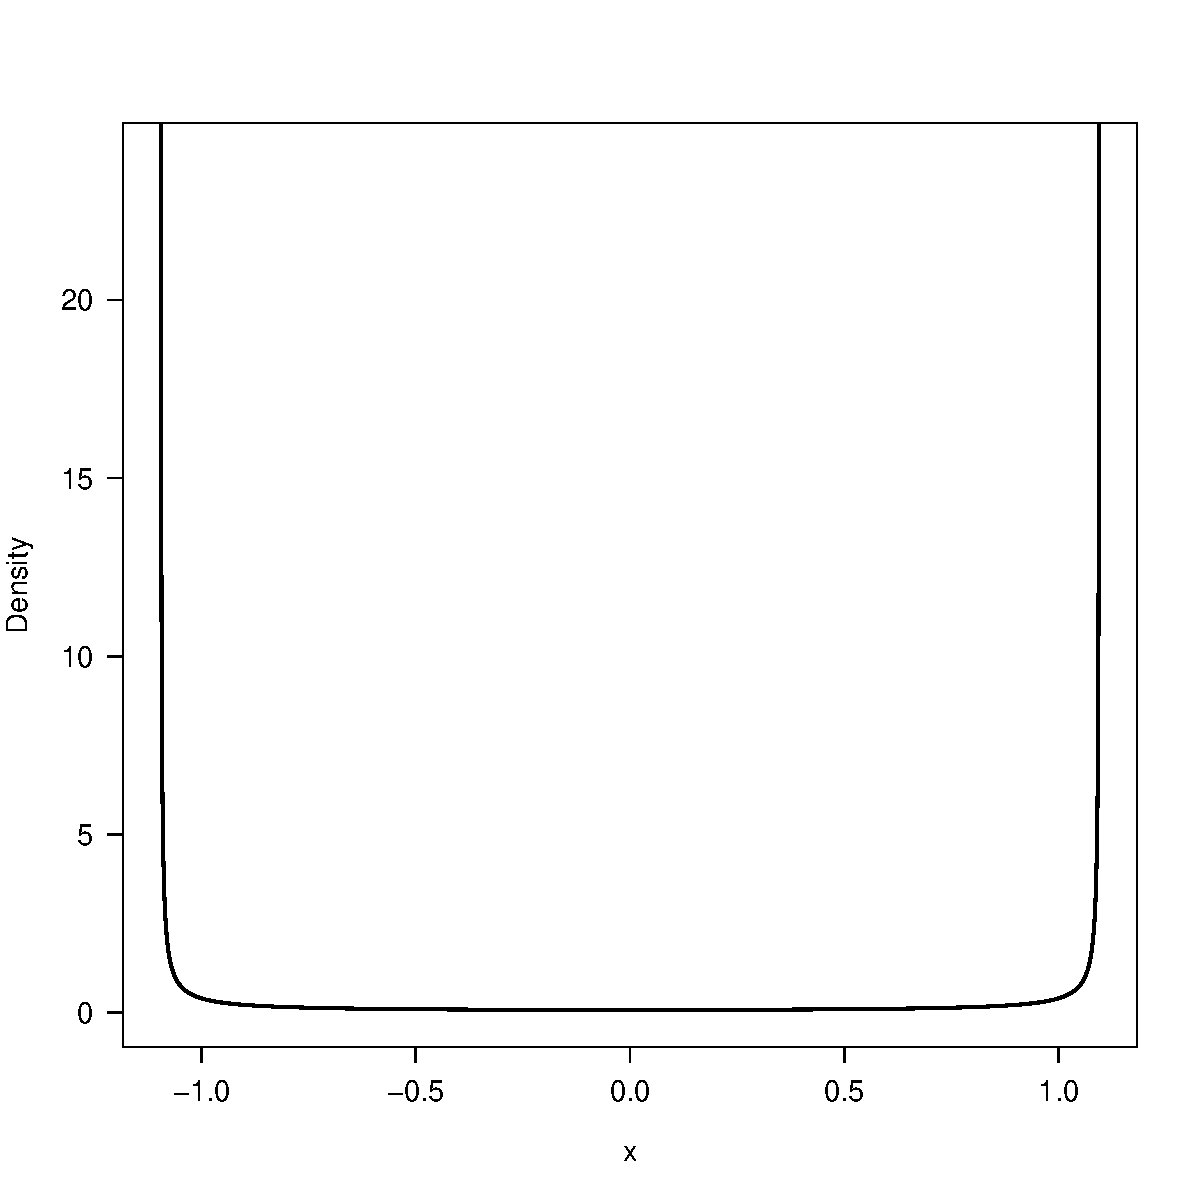
\includegraphics[width=0.46\textwidth]{chunks/beta}}
	\subfigure[Gamma distribution]{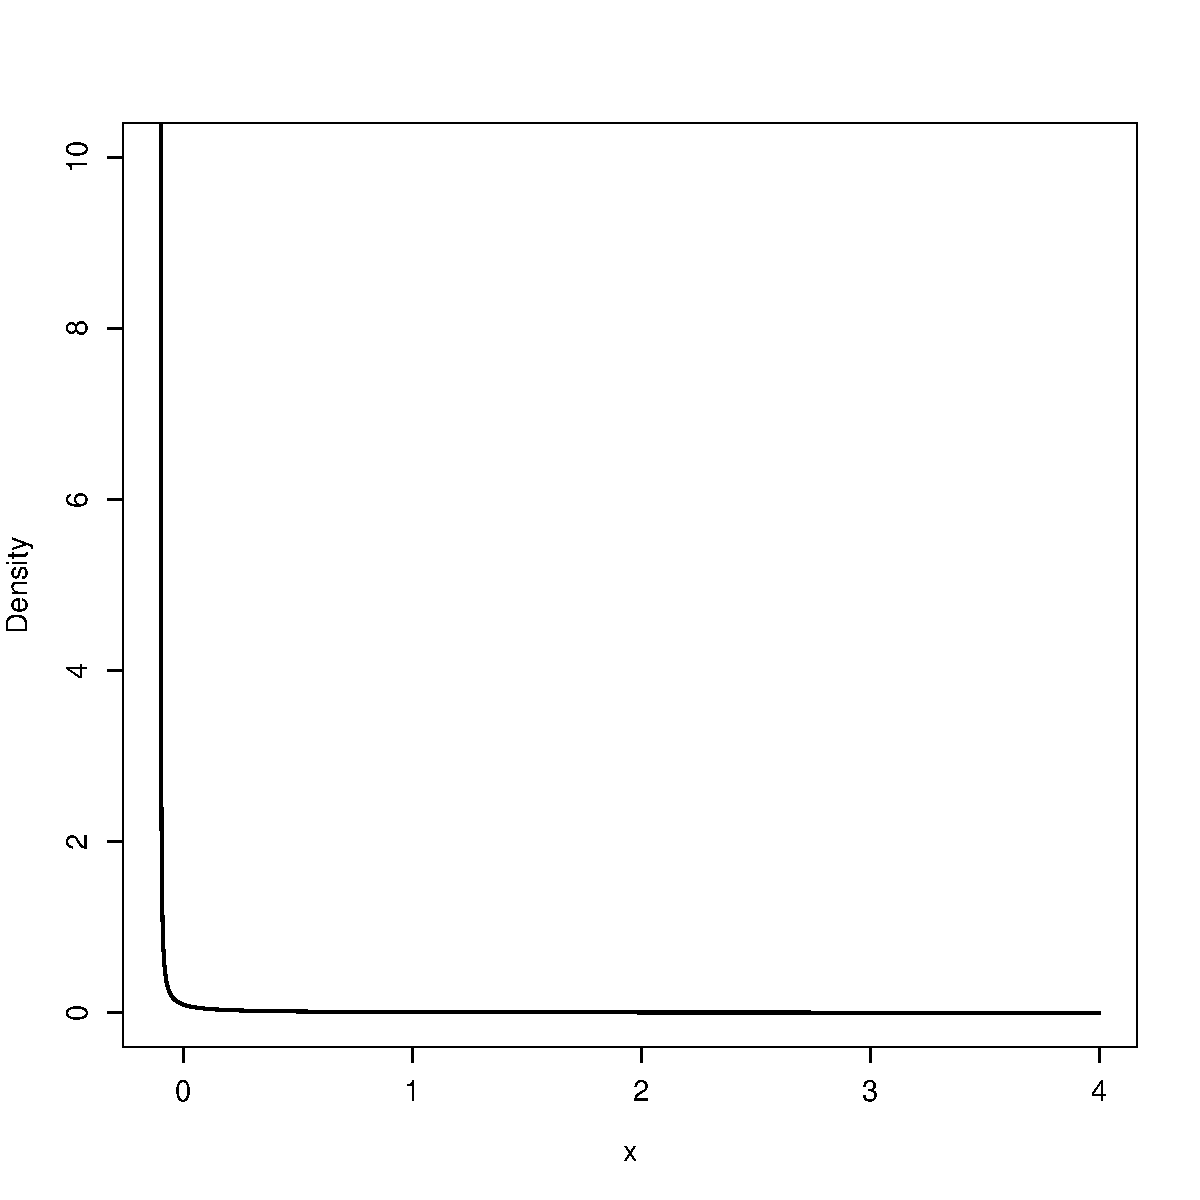
\includegraphics[width=0.46\textwidth]{chunks/gamma}}
	\caption{Rescaled $\textrm{Beta}(1/10, 1/10)$ and $\textrm{Gamma}(1/100, 1/100)$ distributions with variance $1$ and mean $0$.}
	\label{fig::distributions}
\end{figure}

\item Scaled and centered Beta distribution with $\alpha=\beta=1/10$. This is a bimodal distribution with a lot of weight placed on the modes. See the left of Figure \ref{fig::distributions}.
\item Scaled and centered Gamma distribution with $\alpha=\beta=1/100$. This is asymmetric and with heavy tails. See the right of Figure \ref{fig::distributions}.
\end{enumerate}

I have chosen $5$ degrees of freedom for the $t$-distribution since it is the first integer degree of freedom where $t$ has finite fourth moment, recall Theorem \ref{thm:asymptotics} (ii). The parameters for the Beta and Gamma make them both extreme, as should be clear from Figure \ref{fig::distributions}. I have chosen these distributions since I believe they are likely to make t

Table \ref{tab:simulation} contains $100 \times \MSE_\alpha/\MSE_{\alpha_s}$. Values higher than $100$ are in favor of $\widehat{\alpha}_s$ and values lower than $100$ in favor of $\widehat{\alpha}$. The table shows that $\alpha_s$ tends to outperform $\alpha$ when both $k$ and $n$ is large and and $\sigma$ is small, but with no clear trends otherwise. In this simulation $\widehat{\alpha}_s$ does slightly better than $\widehat{\alpha}$, the geometry mean of $\MSE_\alpha/\MSE_{\alpha_s}$ is $1.08$, given an $8$\% advantage to $\widehat{\alpha}_s$. Of course, this is a small simulation study and it is hard to predict what would happen with other distributions. Still, I believe the result of these simulations should be counted in favor of sample standardized alpha.

To sum up, sample alpha won the maximum likelihood and robustness competitions, drew the asymptotic efficiency competition, and lost the finite sample competition. The tally is sample alpha 2\sfrac{1}{2} - 1\sfrac{1}{2} standardized alpha. 

%% <<<<< Example table start (\label{tab:reliabilites})
% latex table generated in R 3.6.2 by xtable 1.8-4 package
% Mon Feb 03 15:19:37 2020
\begin{table}[ht]
\centering
\caption{Simulations of $100 \times \textrm{MSE}_\alpha/\textrm{MSE}_{\alpha_s}$ in the parallel model} 
\begin{tabular}{rlllllllll}
    & $t(5)$ & $t(5)$ & $t(5)$ & Beta & Beta & Beta & Gamma & Gamma & Gamma \\
  & $\sigma = 2$ & $\sigma = 1$ & $\sigma = 0.5$ & $\sigma = 2$ & $\sigma = 1$ & $\sigma = 0.5$ & $\sigma = 2$ & $\sigma = 1$ & $\sigma = 0.5$ \\
$k = 5, n = 50$ & 106 & 112 & 103 & 106 & 112 & 114 & 107 & 105 & 113 \\ 
  $k = 20, n = 50$ & 113 & 105 & 105 & 95.8 & 90.8 & 98.9 & 97.5 & 97.6 & 94.7 \\ 
  $k = 5, n = 200$ & 99.5 & 98.7 & 102 & 101 & 101 & 100 & 74.7 & 60.6 & 67.4 \\ 
  $k = 20, n = 200$ & 37.8 & 174 & 138 & 144 & 82.6 & 308 & 257 & 189 & 153 \\ 
  \end{tabular}
\end{table}
\newcommand{\geomean}{1.08}


%% example table end >>>>>

\section{Argument 2. The issue with standardized scores}
\label{sec:argument 2}
I have two arguments against using standardized alpha for standardized
test items. First, you should not standardize test items. Second,
even if you decide to standardize test items, please avoid standardized
alpha and use a suitably modified congeneric reliability instead.

My point of departure is a quote of \citet[][p.348]{Osburn2000-jd}:

\enquote{However, it is important to note that the true reliability of a measure is the same for both standardized and unstandardized observed scores.}

I will argue against this. Recall the definition of reliability from
section $2$. Given a linear predictor $\hat{Z}$ of $Z$, the
reliability $\omega$ equals the square correlation between $\hat{Z}$
and $Z$, or $\omega=\Cor^{2}(\hat{Z},Z)$. Assume
we know the values of $\lambda$ and $\sigma$. When you use unstandardized
scores, the the predictor of $Z$ is $\hat{Z}=w_{0}\sum_{i=1}^{k}X_{i}$
for some $w_{0}$ (recall Proposition X). When you use standardized
scores, your predictor is $\hat{Z}^{\star}=w_{0}\sum_{i=1}^{k}\sqrt{\lambda^{2}+\sigma^{2}}^{-1}X_{i}$.
These predictors are not the same, and their reliabilites are not
the same either.

This difference matters. An important motivation for using the squared
correlation between $Z$ and $\hat{Z}$ as the definition of a
reliability coefficient is that it allows us to do correction for
attenuation. Let $\hat{Z}_{1},\hat{Z}_{2}$ be two linear
predictors of two latent variables $Z_{1},Z_{2}$ defined in two different
congeneric models. Assume the errors $\epsilon_{1}$ and $\epsilon_{2}$
are uncorrelated. Our goal is to find the correlation $\Cor(Z_{1},Z_{2})$
between the latent variables $Z_{1}$ and $Z_{2}$ using only the
reliabilities $\omega(\hat{Z}_{1})$, $\omega(\hat{Z}_{2})$,
and the observed correlation $\Cor(\hat{Z}_{1},\hat{Z}_{2})$.
Then
\begin{eqnarray*}
\rho=\Cor(\hat{Z}_{1},\hat{Z}_{2}) & = & \frac{\Cov(Z_{1},\hat{Z}_{1})\Cov(Z_{2},\hat{Z}_{2})}{\sqrt{\Var(\hat{Z}_{1})}\sqrt{\Var(\hat{Z}_{2})}}\Cor(Z_{1},Z_{2})\\
 & = & \omega(\hat{Z}_{1})\omega(\hat{Z}_{2})\Cor(Z_{1},Z_{2})
\end{eqnarray*}
and $\Cor(Z_{1},Z_{2})=\Cor(\hat{Z}_{1},\hat{Z}_{2})/\left[\omega(\hat{Z}_{1})\omega(\hat{Z}_{2})\right]$,
the famous Spearman attenuation {[}{[}ref{]}{]} formula.

If you use the standardized sum scores to form one of your scales,
i.e. $\hat{Z}^{\star}=w_{0}\sum_{i=1}^{k}(\lambda_{i}^{2}+\sigma_{i}^{2})^{-1/2}X_{i}$,
using the reliability $\omega$ based on the sum scores would be wrong,
as you would wrongly calculate $\rho'=\omega(\hat{Z}_{1})\omega(\hat{Z}_{2})\Cor(Z_{1},Z_{2})$
instead of the correct $\rho=\omega(\hat{Z}_{1}^{\star})\omega(\hat{Z}_{2})\Cor(Z_{1},Z_{2})$.
You would be off by a factor of $\omega(\hat{Z}_{1}^{\star})/\omega(\hat{Z}_{1})$.

This connection between reliabilities and the choice of predictor
weights is not new, see e.g. Jöreskog, Li. McNeish (1) repeatedly
insists on taking this connection into account. Several authors recommends you use standardized alpha with standardized sum scores. For instance, \citet[][p.451]{Falk2011-ae} states \enquote{If researchers intend to sum
standardized scores, the correlation matrix is more appropriate for determining internal consistency.} Another example is \citet[][p.99]{Cortina1993-aq} \enquote{Standardized alpha is appropriate if item standard scores are summed to form scale scores.}

I will now argue you should never standardized your items. That is, you should avoid $w_{i}=(\lambda_{i}^{2}+\sigma_{i}^{2})^{-1/2}$ when you form your predictor.
Using some $w\ne1$ seems reasonable, for you would not want items
with large variance to overshadow all the other contributions to $\hat{Z}$.
But there is something strange about this particular $w$. Wouldn't
it be just as sensible to use $w=\sigma_{i}^{-1}$? Dividing by $(\sigma_{i}^{2}+\lambda_{i}^{2})^{1/2}$
seems wrong, as you want items with large loadings to have a large
influence on your prediction of $Z$, but dividing by $(\sigma_{i}^{2}+\lambda_{i}^{2})^{1/2}$
makes the influence of large $\lambda_{i}$s smaller. Clearly, $w=\sigma_{i}^{-1}$
does not suffer from this problem. 

Call the reliability with weights $w=\sigma_{i}^{-1}$ the \emph{sigma reliability} and denote it $\omega_\sigma$. Using Proposition \ref{prop:reliability motivation} it can be written as
\begin{equation}
\omega_\sigma=\frac{k\overline{\lambda\sigma^{-1}}^{2}}{k\overline{\lambda\sigma^{-1}}^{2}+1}.\label{eq:Sigma-standardized reliability}
\end{equation}

But while we are at it, why not just use the optimal weights, yielding
coefficient $H$ and the Thurstone factor scores instead of the standardized
alpha and standardized sum scores? \citet{McNeish2019-ea} argue in favour of
adopting optimal weights when forming the predictor.

% The next proposition gives the formulas and optimal weights for the
% four reliability coefficients introduced in this paper. The optimal
% weights satisfy $\omega=1-\MSE \left(\hat{Z}\right)$.
% \begin{prop}
% \label{prop:Z-reliabiltiy}Let $\hat{Z}=\sum_{i=1}^{k}w_{i}X_{i}$ be a linear predictor of $Z$.

% \begin{enumerate}[label=(\roman*)]
% \item The congeneric reliability has weights $w_0 =  \overline{\lambda^{2}}/(k\overline{\lambda}^{2}+\overline{\sigma^{2}})$ and equals
% \begin{equation}
% \tag{\ref{eq:Congeneric reliability}}
% \omega=\frac{k\overline{\lambda}^{2}/\overline{\sigma^{2}}}{k\overline{\lambda}^{2}/\overline{\sigma^{2}}+1}.
% \end{equation}
% \item Coefficient $H$ has weights $w_i =\lambda_{j}/[\sigma_{j}^{2}(1+k\overline{\lambda\sigma^{-2}})]$ and equals
% \begin{equation}
% \tag{\ref{eq:coefficient_H}}
% \omega_{H}=\frac{k\overline{\lambda^{2}\sigma^{-2}}}{k\overline{\lambda^{2}\sigma^{-2}}+1}.
% \end{equation}
% \item The standardized reliability has weights $w=w_{0}(\lambda_{i}^{2}+\sigma_{i}^{2})^{-1/2}$ and equals
% \begin{equation}
% \omega_s=\frac{k\overline{\lambda(\lambda^{2}+\sigma^{2})^{-1/2}}^{2}/\overline{\sigma^{2}(\lambda^{2}+\sigma^{2})^{-1}}}{k\overline{\lambda(\lambda^{2}+\sigma^{2})^{-1/2}}^{2}/\overline{\sigma^{2}(\lambda^{2}+\sigma^{2})^{-1}}+1}.
% \end{equation}
% \item The sigma reliability has weights $w=w_{0}\sigma_{i}^{-1}$ and equals
% \begin{equation}
% \omega_\sigma=\frac{k\overline{\lambda\sigma^{-1}}^{2}}{k\overline{\lambda\sigma^{-1}}^{2}+1}.\label{eq:Sigma-standardized reliability}
% \end{equation}
% \end{enumerate}
% \end{prop}
% \begin{proof}
% See the appendix, page \pageref{proof:Z-reliability}.
% \end{proof}

No one would use the standardized reliability \eqref{eq:Standardized reliability}
or the sigma reliability \eqref{eq:Sigma-standardized reliability}
if $\sigma_{i}^{2}=\sigma^{2}$ for all $i$. The following theorem
exposes a basic fact about these three reliability coefficients:
\begin{thm}
\label{thm:Properties of three} Assume the $\tau$-equivalent model,
i.e. the congeneric model with $\lambda_{i}=\lambda>0$ for all $i$
but possibly different residual errors $\sigma_{i}$. Let $\omega$ be the congeneric
reliability \eqref{eq:Congeneric reliability}, $\omega_{s}$ the standardized reliability \eqref{eq:Standardized reliability},
$\omega_{\sigma}$ the sigma reliability \eqref{eq:Sigma-standardized reliability},
and $\omega_{H}$ coefficient $H$ \eqref{eq:coefficient_H}. 

\begin{enumerate}[label=(\roman*)]
\item Assume the $\tau$-equivalent model,
i.e. the congeneric model with $\lambda_{i}=\lambda>0$ for all $i$
but possibly different residual errors $\sigma_{i}>0$. Then
\[
\omega_{h}\geq\omega_{\sigma}\geq\omega_{s}\geq\omega,
\]
with all inequalities strict unless $\sigma_{i}=\sigma$ or all
$i$. In that case, $\omega_{h} = \omega_{\sigma} = \omega_{s} = \omega$.
\item Assume the congeneric model with $\sigma_i = \sigma > 0$ for all $i$ but possibly different loadings $\lambda_i$. Then
\[
\omega_{H}\geq\omega_{\sigma}=\omega\geq\omega_{s},
\]
and the inequalities are strict unless $\lambda_{i}=\lambda$ for all
$i$. In that case, $\omega_{h} = \omega_{\sigma} = \omega_{s} = \omega$.

\end{enumerate}

\end{thm}
\begin{proof}
See the appendix, page \pageref{proof:Properties}.
\end{proof}
You can interpret Theorem \ref{thm:Properties of three} as a ranking factor scores too. It says
regression scores are better than $\sigma$-standardized sum scores,
which in turn are better than the standardized sum scores, which are
better than the ordinary sum scores.

% We can use the expressions of Proposition \ref{prop:Z-reliabiltiy}
% to compare the effect of $\hat{Z}$ on the reliability of our
% measurements.

Since coefficient $H$ uses the optimal weights, it is guaranteed to
be larger than the three other reliabilities mentioned above. The
other three reliabilities can be in any order, but will usually follow
$\omega_{\sigma}$ will usually be the largest, sometimes . In a short
simulation ($10^{5}$ repetitions) of $k=5$ items with $\lambda_{i}\sim \textrm{Exp}(1)$
and $\sigma_{i}\sim \textrm{Exp}(1)$ independently with $i=1,\ldots,5$, $\omega_{\sigma}$
was the largest $0.98\%$ of the time, $\omega$ largest $0.02\%$
of the time, but $\omega_{s}$ was never the largest ($\omega_{s}>\omega_{\sigma}$
happened though). The congeneric $\omega$ dominated $\omega_{s}$
in $6$ of $10$ iterations. You could argue this simulation study
is somewhat unrealistic: In a slightly different simulation with $\lambda_{i}^{2}\sim N(0,1)$
and $\sigma_{i}\sim \textrm{HalfNormal}(0,1)$, $\omega_{\sigma}$ was the
largest $0.92\%$ of the time and $\omega_{s}>\omega$ a nice $70\%$
of the time. Again, $\omega_{s}$ was never the largest, which suggest
it cannot be larger than both $\omega$ and $\omega_{\sigma}$ at
the same time. The take-away from these two simulation studies is
that $\omega_{\sigma}$ generally does better than $\omega_{s}$ and
$\omega$, while it is hard to predict the winner among $\omega$
and $\omega_{s}$. 

\begin{example}
%% <<<<< Example table start (\label{tab:reliabilites})
% latex table generated in R 4.0.0 by xtable 1.8-4 package
% Thu May 14 11:11:44 2020
\begin{table}[ht]
\centering
\caption{Comparison of reliability coefficients on personality data} 
\label{tab:reliabilites}
\begin{tabular}{lccccc}
  \toprule
 & A & C & E & N & O \\ 
  \cmidrule{1-6}
Congeneric reliability ($R$) & 0.712 & 0.733 & 0.767 & 0.813 & 0.610 \\ 
  Coefficient \it{H} ($R_H$) & 0.765 & 0.739 & 0.778 & 0.850 & 0.651 \\ 
  Standardized reliability ($R_S$) & 0.724 & 0.734 & 0.763 & 0.815 & 0.618 \\ 
  Sigma reliability ($R_\sigma$) & 0.744 & 0.736 & 0.770 & 0.836 & 0.630 \\ 
   \bottomrule
\end{tabular}
  \vskip7.0pt
A, agreeableness; C, conscientiousness; E, extraversion; N, neuroticism; O, openness to experience 
\end{table}

%% example table end >>>>>

In this example we will take a look at the data set $\texttt{bfi}$ from he $\texttt{R}$ \citep{Team2013-tt} package $\texttt{psychTools}$ \citep{Revelle2019-te}. This data set contains the responses on $25$ personality self report items from the International Personality Item Pool \citep{Goldberg1999-iz} collected from the Synthetic Aperture Personality Assessment project \citep{Revelle2016-ez}. The $25$ items are evenly distributed across the big five traits: Agreeableness, conscientiousness, extraversion, neuroticism, and openness to experience. 

For each trait I estimated the factor loadings $\lambda$ and residual standard deviations $\sigma$ in the congeneric measurement model \eqref{eq:one-factor model} using  $\texttt{lavaan}$ \citep{Rosseel2012-yg}. I plugged these estimates into the definitions of the four reliability coefficients. The results are in Table \ref{tab:reliabilites}. As expected, $\omega_\sigma$ is larger than both $\omega_s$ and $\omega$ for all five traits. Moreover, $\omega_s > \omega$ for all traits except extraversion, where the difference is marginal. 
\end{example}

My second argument against $(\lambda_{i}^{2}+\sigma_{i}^{2})^{-1}$
follows \citep{Falk2011-ae}. The assumptions of a $\tau$-equivalent model are hard
to justify to begin with, and unlikely to be true. By Proposition \ref{prop:weighted alpha}, the standardized coefficient alpha equals the standardized reliability only when the modified model
\[
X_{i}^{\star}=\frac{\lambda_{i}}{\sqrt{\lambda_{i}^{2}+\sigma_{i}^{2}}}Z+\frac{\sigma_{i}}{\sqrt{\lambda_{i}^{2}+\sigma_{i}^{2}}}\epsilon_{i}\:i=1,\ldots,k
\]
is $\tau$-equivalent. This occurs if and only if each $\lambda_{i}/(\lambda_{i}^{2}+\sigma_{i}^{2})=\lambda^{\star}$
for some $\lambda^{\star}$, that is, when all standardized factor loadings are equal. Of course, this would be an exceptional coincidence. To avoid this unwarranted assumption, use structural equation modeling to estimate $\lambda_{i},\sigma_{i}$, and plug them into
the formula for the standardized reliability $\omega_s$ \eqref{eq:Standardized reliability}. 

(Have a short simulation here?)

To recap, my arguments are: (i) You should neither avoid standardization altoghether nor standardizee with $(\lambda_{i}^{2}+\sigma_{i}^{2})^(-1/2)$ nor $1$. You should standardize with $\sigma_i^{-1}$ or use the optimal weights, as this yields better results in the most plausible scenarios. (ii) Even if you decide to standardize with $(\lambda_{i}^{2}+\sigma_{i}^{2})^{-1/2}$, please avoid standardized alpha, as won't equal $\omega_s$ under any reasonable assumptions.

% This observation also counters a possible, but wrong, interpretation
% of Proposition \ref{thm:Properties of three}. For $\omega_{s}>\omega$
% under the $\tau$-equivalent model by Proposition \ref{thm:Properties of three} and $\alpha = \omega$ under the $\tau$-equivalent model. Then it seems reasonable to use standardized alpha together with the sum scores. After all, standardized alpha
% can be calculated from the covariance matrix alone, and does not require
% any estimation of $\lambda$ and $\sigma$. But this is wrong! For
% as mentionioned, $\alpha_{s}=\omega_{s}$ only when $\lambda_{i}/(\lambda_{i}^{2}+\sigma_{i}^{2})=\lambda$.
% Otherwise, $\alpha_{s}<\omega_{s}$ by Propositon 1.

% \subsection*{Digression: The sigma alpha coefficient}
% Both coefficient alpha and standardized alpha are simple functions
% of the covariance matrix $\Sigma$, but the reliability coefficients
% in Proposition \ref{prop:Z-reliabiltiy} are not simple functions
% of $\Sigma$ except under exceptional circumstances such as $\tau$-equivalence.
% Everything else being equal, simple solutions should be preferred
% over complex solutions. Arguments in favor of coefficient alpha along
% these lines are common, see e.g. {[}{[}ref; take 2 with page numbers.{]}{]}.

% Since $\omega$ has $\alpha$ and $\omega_{s}$ has $\alpha_{s}$,
% the sigma reliability \eqref{eq:Sigma-standardized reliability} should
% its own alpha coefficient as well. Here I understand an alpha coefficient
% as a closed form function of the covariance matrix $\Sigma$ such
% that $\alpha\left(\Sigma\right)=\omega$ {[}{[}fill in{]}. Now it
% is time to derive it. The covariance matrix $\Sigma$ under the $\tau$-equivalent
% model has diagonal elements $\lambda^{2}+\sigma_{i}^{2}$ and off-digonal
% elements $\lambda^{2}$. Then $\lambda^{2}=\left(k-1\right)^{-1}\left(\mathbf{i}^{T}\Sigma\mathbf{i}/k-\tr\Sigma/k\right)$
% and $\sigma^{2}=\diag\Sigma-\lambda^{2}$. Define the sigma standardized
% matrix
% \begin{eqnarray*}
% \Xi & = & \diag\sigma^{-1}\Sigma\diag\sigma^{-1},
% \end{eqnarray*}
% and the sigma coefficient alpha (sigma alpha for short) as
% \begin{eqnarray}
% \alpha_{\sigma} & = & \frac{k}{k-1}\left(1-\frac{\tr\Xi}{\mathbf{i}^{T}\Xi\mathbf{i}}\right)\label{eq:alpha_sigma-1}
% \end{eqnarray}
% The sigma alpha is only interesting when $\alpha_{\sigma}=\omega_{\sigma}$,
% or at the very least when $\alpha_{\sigma}\approx\omega_{\sigma}$.
% By the reasoning of Proposition 1, $\alpha_{\sigma}=\omega_{\sigma}$
% under the congeneric model only when 
% \begin{equation}
% X_{i}^{\star}=\frac{\lambda_{i}}{\sigma_{i}}Z+\epsilon_{i}\:i=1,\ldots,k\label{eq:sigma model}
% \end{equation}
% is $\tau$-equivalent. In other words, $\alpha_{\sigma}=\omega_{\sigma}$
% only when every standardized factor loading is the same, or $\lambda_{i}/\sigma_{i}=\lambda^{\star}$
% for some $\lambda^{\star}$. From Proposition \ref{prop:Z-reliabiltiy}
% (iii) and (ii) $\alpha_{\sigma}=\omega_{\sigma}=\omega_{H}$ in this
% case.

% Sadly, condition \eqref{eq:sigma model} renders $\alpha_{\sigma}=\omega_{\sigma}$
% trivial. By the definition of $\omega_{\sigma}$ \eqref{eq:Sigma-standardized reliability},
% $\omega_{k}=k/\left(k+1\right)$ when \eqref{eq:sigma model} holds, no matter what values of $\lambda$ and $\sigma$.
% Moreover, some elements of $\diag\Sigma-\lambda^{2}$ may be less
% than $0$ when $\Sigma$ fails to correspond to a $\tau$-equivalent model, which makes the undefined. Since this happens with probability $1$ when $S$ is used in place of $\Sigma$, $\widehat{\alpha}_{\sigma}$
% is a likely to be horrible estimator of $\omega_{s}$. Instead,
% estimate $\omega_{\sigma}$ using the plug-in principle estimator
% $\widehat{\omega}_{\sigma}$, where estimates of $\lambda$ and $\sigma$
% can be calculated using e.g. $\texttt{lavaan}$. To calculate confidence
% intervals for this quantity, you can use either the delta method,
% the parametric boostrap, or the non-parametric bootstrap.

\section{Remarks}
\label{sec:remarks}
In some cases you cannot access the sample covariance matrix $S$. Then coefficient alpha is unavailable. If you can get hold of the correlation matrix $R$ the standardized alpha might be the best you can do. An example of this scenario is $R$ is a polychoric correlation matrix.

There remains an argument in favor using correlation matrices when calculating the congeneric reliability coefficient. Consider the case when the sample correlation matrix $R$ is not the correlation matrix derived from the sample covariance matrix $S$, but rather the polychoric correlation matrix $\Theta$ \citep{Olsson1979-ti}. Assume the observed $X$ are scored on a discrete and ordinal scale, for instance on a Likert scale. In this case, some authors argue we should use the polychoric correlation matrix $\Theta$ instead of the sample covariance matrix $S$. 

\citet[][p. 415]{McNeish2018-vu} argues the sample covariance matrix is biased towards $0$ in these circumstances, and presumably that the sample alphas will have a large mean squared error. He proposes to overcome this problem by using the polychoric correlation as an estimator of the correlation of $X$:
\begin{displayquote}To accommodate items that are not on a continuous scale, the
covariances between items can instead be estimated with a polychoric covariance (or correlation) matrix rather than with a Pearson covariance matrix.
\end{displayquote}
This argument is fallacious since the polychoric correlation does not estimate the correlation matrix of $X$, but the correlation matrix of some hypothetical unobserved $Y$ that generate the observed $X$ using a discretization procedure. These correlation matrices are not the same in general. 

Acknowledging this, \citet[][p.2]{Gadermann2012-jl} (and, indirectly, \citet{Zumbo2007-ap}) claim we are truly interested in the covariance matrix of the latent variables $Y$ that generate the observed $X$s using a discretization procedure. Recall from section \ref{sec:coefficienta alpha} that each reliability coefficient has an associated predictor $\hat{Z}$ of $Z$. This predictor can only be based on the available data, namely $X$. Since predictors based on $Y$ cannot be computed as $Y$ is unknown, the predictive performance of this method has no practical importance. For instance, correction for attenuation is impossible to use when coefficient alpha is based on the polychoric correlation. For you would not be able to calculate the correlation between any prediction of $Z$ based on $Y$ and some other variable $U$ when $Y$ is unknown.

When we estimate $\rho^{2}(\hat{Z},Z)$, the weights
$w$ are already known, as we use them to form the predictor $\hat{Z}$.
The parameters $\lambda_{i}$ and $\sigma_{i}$ are not known though.
This means we should not be interested in estimating and doing inference
on a theoretical $\rho^{2}$ when $\hat{Z}$ has some optimal
weights, but rather $\rho^{2}$ when $\hat{Z}$ has some fixed
but estimated weights. In the correction for attenuation problem
above, $\Cor(\hat{Z}_{1},\hat{Z}_{2})$ cannot
be estimated without forming the predictors $\hat{Z}_{1}$ and
$\hat{Z}_{2}$. In this case we also want to estimate the correlation
between $\Cor(\hat{Z}_{1},\hat{Z}_{2})$ for fixed
$w_{1},w_{2}$, not the correlation for the optimal $w_{1}$ and $w_{2}$. \citet{Chalmers2018-fj} made similar points and 

\section{Appendix}

\begin{proof}[Proof of Proposition \ref{prop:reliability motivation}]\label{proof:reliability motivation}
Since $\Var Z=1$, the covariance between $\hat{Z}$ and $Z$
is
\begin{eqnarray*}
\Cov\left(Z,\hat{Z}\right)=\Cov\left[Z,\sum_{i=1}^{k}w_{i}\left(Z\lambda_{i}+\sigma_{i}\epsilon\right)\right] & = & \sum_{i=1}^{k}w_{i}\lambda_{i}.
\end{eqnarray*}
and the variance of $\hat{Z}$ is
\[
\Var\left(\hat{Z}\right)=\Var\left[\sum_{i=1}^{k}w_{i}\left(Z\lambda_{i}+\sigma_{i}\epsilon\right)\right]=\left(\sum_{i=1}^{k}w_{i}\lambda_{i}\right)^{2}+\sum_{i=1}^{k}w_{i}^{2}\sigma_{i}^{2}.
\]
Combining these two formulas gives us the squared correlation between
$Z$ and $\hat{Z}$,
\begin{eqnarray*}
\omega=\Cor^{2}\left(\hat{Z},Z\right) & = & \frac{\left(\sum_{i=1}^{k}w_{i}\lambda_{i}\right)^{2}}{\left(\sum_{i=1}^{k}w_{i}\lambda_{i}\right)^{2}+\sum_{i=1}^{k}w_{i}^{2}\sigma_{i}^{2}}.
\end{eqnarray*}

For the second claim,
\begin{eqnarray*}
E\left\{ \left[Z-\sum_{i=1}^{k}w_{i}\left(\lambda_{i}Z+\sigma_{i}\epsilon_{i}\right)\right]^{2}\right\}  & = & E\left\{ \left[Z-\sum_{i=1}^{k}w_{0}w_{i}\left(\lambda_{i}Z+\sigma_{i}\epsilon_{i}\right)\right]^{2}\right\} ,\\
 &  & w_{0}^{2}\sum_{i=1}^{k}w_{i}^{2}\sigma_{i}^{2}+\left(w_{0}\sum_{i=1}^{k}w_{i}\lambda_{i}-1\right)^{2}.
\end{eqnarray*}
Differentiate with respect to $w_{0}$ to find the minimizer
\[
w_{0}=\frac{\sum_{i=1}^{k}w_{i}\lambda_{i}}{\left(\sum_{i=1}^{k}w_{i}^{2}\sigma_{i}^{2}+\left(\sum_{i=1}^{k}w_{i}\lambda_{i}\right)^{2}\right)}
\]
And then
\[
E\left\{ \left[Z-\sum_{i=1}^{k}w_{i}\left(\lambda_{i}Z+\sigma_{i}\epsilon_{i}\right)\right]^{2}\right\} =\frac{\left(\sum_{i=1}^{k}w_{i}\lambda_{i}\right)^{2}}{\left(\sum_{i=1}^{k}w_{i}\lambda_{i}\right)^{2}+\sum_{i=1}^{k}w_{i}^{2}\sigma_{i}^{2}}
\]
as claimed.
\end{proof}


\begin{proof}[Proof of Proposition \ref{prop:weighted alpha}]
\label{proof:weighted alpha}Clearly $wX$ is $\tau$-equivalent
if and only if $w_{i}\lambda_{i}=w_{j}\lambda_{j}$ for each $i,j$,
which implies $w^{T}\lambda=k\lambda_{i}w_{i}$. Then
\begin{eqnarray*}
\alpha_{w} & = & \frac{k}{k-1}\left(1-\frac{w^{T}\diag\Sigma w}{w^{T}\Sigma w}\right)\\
 & = & \frac{k}{k-1}\left(\frac{k^{2}\lambda_{1}^{2}w_{1}^{2}-k\lambda_{1}^{2}w_{1}^{2}}{k^{2}\lambda_{1}^{2}w_{1}^{2}+\sum_{i=1}^{k}w_{i}^{2}\sigma_{i}^{2}}\right)\\
 & = & \frac{(w^{T}\lambda)^{2}}{(w^{T}\lambda)^{2}+w^{T}\Psi w}
\end{eqnarray*}
as claimed.
\end{proof}


This lemma comes in handy in the proof of Proposition \ref{prop:Reliabilities.} as it allows us to use Jensen's inequality.

\begin{lem}
Assume the congeneric model of \eqref{eq:one-factor model} and let $\alpha$ be as in \eqref{eq:Coefficient alpha} and $\alpha_s$ be as in \eqref{eq:standardized alpha}. Then $\alpha_{s}\geq\alpha$
if and only if
\begin{equation}
\label{eq:alpha_s_alpha_inequality}
\sum_{i\neq j}\frac{\lambda_{i}\lambda_{j}}{\sqrt{\sigma_{i}^{2}+\lambda_{i}^{2}}\sqrt{\sigma_j^{2}+\lambda_{j}^{2}}} 
\geq
\sum_{i\neq j}\frac{\lambda_{i}\lambda_{j}}{\sum_{i=1}^{k}\left(\lambda_{i}^{2}+\sigma_{i}^{2}\right)/k}
\end{equation}
\end{lem}

\begin{proof}
From definition \eqref{eq:Coefficient alpha}
\begin{eqnarray*}
\alpha_{s} & = & \frac{k}{k-1}\left(1-\frac{k}{\mathbf{i}^{T}\Phi\mathbf{i}}\right)\\
 & = & \frac{k}{k-1}\left(1-\frac{k}{\sum_{i\neq j}\frac{\lambda_{i}\lambda_{j}}{\sqrt{\sigma_{i}^{2}+\lambda_{i}^{2}}\sqrt{\sigma_{j}^{2}+\lambda_{j}^{2}}}+k}\right)
\end{eqnarray*}
and definition \eqref{eq:standardized alpha}
\begin{eqnarray*}
\alpha & = & \frac{k}{k-1}\left(1-\frac{\tr\Sigma}{\mathbf{i}^{T}\Sigma\mathbf{i}}\right)\\
 & = & \frac{k}{k-1}\left(1-\frac{\sum_{i=1}^{k}\left(\sigma_{i}^{2}+\lambda_{i}^{2}\right)}{\sum_{i\neq j}\lambda_{i}\lambda_{j}+\sum_{i=1}^{k}\left(\sigma_{i}^{2}+\lambda_{i}^{2}\right)}\right)
\end{eqnarray*}
Thus $\alpha_{s}\geq\alpha$ if and only if
\[
\frac{k}{\sum_{i\neq j}\frac{\lambda_{i}\lambda_{j}}{\sqrt{\sigma_{i}^{2}+\lambda_{i}^{2}}\sqrt{\sigma_{j}^{2}+\lambda_{j}^{2}}}+k}\leq\frac{\sum_{i=1}^{k}\left(\sigma_{i}^{2}+\lambda_{i}^{2}\right)}{\sum_{i\neq j}\lambda_{i}\lambda_{j}+\sum_{i=1}^{k}\left(\sigma_{i}^{2}+\lambda_{i}^{2}\right)}
\]
which happens if and only if 
\[
\sum_{i\neq j}\frac{\lambda_{i}\lambda_{j}}{\sqrt{\sigma_{i}^{2}+\lambda_{i}^{2}}\sqrt{\sigma_j^{2}+\lambda_{j}^{2}}}\geq\sum_{i\neq j}\frac{\lambda_{i}\lambda_{j}}{\sum_{i=1}^{k}\left(\lambda_{i}^{2}+\sigma_{i}^{2}\right)/k}
\]
\end{proof}

\begin{proof}[Proof of Proposition \ref{prop:Reliabilities.}]\label{proof:Reliabilities.}
We start with (i), where
\begin{eqnarray*}
\alpha & = & \frac{k}{k-1}\left(1-\frac{\textrm{tr}\Sigma}{\mathbf{i}^{T}\Sigma\mathbf{i}}\right)\\
 & = & \frac{k}{k-1}\left(1-\frac{\sum_{i=1}^{k}\left(\sigma_{i}^{2}+\lambda_{i}^{2}\right)}{\sum_{i\neq j}\lambda_{i}\lambda_{j}+\sum_{i=1}^{k}\left(\sigma_{i}^{2}+\lambda_{i}^{2}\right)}\right)\\
 & = & \frac{k}{k-1}\left(\frac{k\overline{\lambda}^{2}-\overline{\lambda^{2}}}{k\overline{\lambda}^{2}+\overline{\sigma^{2}}}\right)\\
 & = & \frac{k\overline{\lambda}^{2}}{k\overline{\lambda}^{2}+\overline{\sigma^{2}}}-\left(\frac{\overline{\lambda^{2}}-\overline{\lambda}^{2}}{k\overline{\lambda}^{2}+\overline{\sigma^{2}}}\right)\\
 & = & \omega-\left(\frac{\overline{\lambda^{2}}-\overline{\lambda}^{2}}{k\overline{\lambda}^{2}+\overline{\sigma^{2}}}\right)
\end{eqnarray*}
Since $(\overline{\lambda^{2}}-\overline{\lambda}^{2})/(k\overline{\lambda}^{2}+\overline{\sigma^{2}})\geq0$
and equals $0$ if and only if all $\lambda$s are equal by Jensen's inequality, $\alpha=\omega$
iff all $\lambda$s are equal and is otherwise an underestimate.

(ii) From \eqref{eq:Alpha-alpha_s inequality} and $\lambda_{i}=\lambda$
for all $i$, we need to show
\[
\lambda^{2}\sum_{i\neq j}\frac{1}{\sqrt{\sigma_{i}^{2}+\lambda^{2}}\sqrt{\sigma_{j}^{2}+\lambda^{2}}}\geq\lambda^{2}\sum_{i\neq j}\frac{1}{\sum_{i=1}^{k}\left(\lambda^{2}+\sigma_{i}^{2}\right)/k}
\]
Recall Jensen's inequality: When $f$ is convex, $E\left[f\left(X\right)\right]\geq f\left[E\left(X\right)\right]$ with equality if and only if $f$ is linear.
The function $f\left(x,y\right)=\left(x+\lambda^{2}\right)^{-1/2}\left(y+\lambda^{2}\right)^{-1/2}$
is convex for any $\lambda$. Let $E\left(X,Y\right)=\left[k\left(k-1\right)\right]^{-1}\left(\sum_{i\neq j}x_{i},\sum_{i\neq j}y_{i}\right)$
and observe that
\begin{eqnarray*}
f\left(E\left(\sigma^{2},\sigma^{2}\right)\right) & = & f\left(\left[k\left(k-1\right)\right]^{-1}\sum_{i\neq j}\sigma_{i}^{2},\left[k\left(k-1\right)\right]^{-1}\sum_{i\neq j}\sigma_{i}^{2}\right)\\
 & = & \left[\left[k\left(k-1\right)\right]^{-1}\sum_{i\neq j}\sigma_{i}^{2}+\lambda^{2}\right]^{-1/2}\left[\left[k\left(k-1\right)\right]^{-1}\sum_{i\neq j}\sigma_{i}^{2}+\lambda^{2}\right]^{-1/2}\\
 & = & \left(\sum_{i=1}^{k}\left(\lambda^{2}+\sigma_{i}^{2}\right)/k\right)^{-1}
\end{eqnarray*}
and by Jensen's inequality
\[
\sum_{i\neq j}\frac{1}{\sqrt{\sigma_{i}^{2}+\lambda^{2}}\sqrt{\sigma_{j}^{2}+\lambda^{2}}}\geq\sum_{i\neq j}\frac{1}{\sum_{i=1}^{k}\left(\lambda^{2}+\sigma_{i}^{2}\right)/k}
\]
with equality if and only if $\sigma_{i}^{2}=\sigma_{j}^{2}$ for
all $i,j$. Since \eqref{eq:Alpha-alpha_s inequality} is true when
$\lambda=0$ too we are done.

As for (iii), from the proof of (i) and (ii) observe that $\alpha_{s}\geq\alpha$
if and only if
\begin{equation}
\label{eq:Alpha-alpha_s inequality}
\frac{k}{\sum_{i\neq j}\frac{\lambda_{i}\lambda_{j}}{\sqrt{\sigma_{i}^{2}+\lambda_{i}^{2}}\sqrt{\sigma_{j}^{2}+\lambda_{j}^{2}}}+k}\leq\frac{\sum_{i=1}^{k}\left(\sigma_{i}^{2}+\lambda_{i}^{2}\right)}{\sum_{i\neq j}\lambda_{i}\lambda_{j}+\sum_{i=1}^{k}\left(\sigma_{i}^{2}+\lambda_{i}^{2}\right)}
\end{equation}
Let $k=2$. Then \eqref{eq:Alpha-alpha_s inequality} simplifies to
\[
\frac{1}{\frac{\lambda_{1}\lambda_{2}}{\sqrt{\left(\sigma_{1}^{2}+\lambda_{1}^{2}\right)\left(\sigma_{2}^{2}+\lambda_{2}^{2}\right)}}+1}\leq\frac{\left(\lambda_{1}^{2}+\sigma_{1}^{2}\right)+\left(\lambda_{2}^{2}+\sigma_{2}^{2}\right)}{2\lambda_{1}\lambda_{2}+\left(\lambda_{1}^{2}+\sigma_{1}^{2}\right)+\left(\lambda_{2}^{2}+\sigma_{2}^{2}\right)}
\]
and further to
\begin{eqnarray*}
\frac{\sqrt{\left(\sigma_{1}^{2}+\lambda_{1}^{2}\right)\left(\sigma_{2}^{2}+\lambda_{2}^{2}\right)}}{\lambda_{1}\lambda_{2}+\sqrt{\left(\sigma_{1}^{2}+\lambda_{1}^{2}\right)\left(\sigma_{2}^{2}+\lambda_{2}^{2}\right)}} & \geq & \frac{\left[\left(\lambda_{1}^{2}+\sigma_{1}^{2}\right)+\left(\lambda_{2}^{2}+\sigma_{2}^{2}\right)\right]/2}{\lambda_{1}\lambda_{2}+\left[\left(\lambda_{1}^{2}+\sigma_{1}^{2}\right)+\left(\lambda_{2}^{2}+\sigma_{2}^{2}\right)\right]/2}
\end{eqnarray*}
By the inequality of arithmetic and geometric means, $1/2\left[\left(\lambda_{1}^{2}+\sigma_{1}^{2}\right)+\left(\lambda_{2}^{2}+\sigma_{2}^{2}\right)\right]\geq\sqrt{\left(\sigma_{1}^{2}+\lambda_{1}^{2}\right)\left(\sigma_{2}^{2}+\lambda_{2}^{2}\right)}$
with equality only if $\lambda_{1}^{2}+\sigma_{1}^{2}=\lambda_{2}^{2}+\sigma_{2}^{2}$.

Consider the second claim of (iii). Let $k>2$ and assume all $\lambda_{j}=0$
except $\lambda_{1},\lambda_{2}$. By \eqref{eq:Alpha-alpha_s inequality}, $\alpha_s \geq \alpha$ if and
only if
\[
\frac{k}{2\frac{\lambda_{1}\lambda_{2}}{\sqrt{\sigma_{1}^{2}+\lambda_{1}^{2}}\sqrt{\sigma_{1}^{2}+\lambda_{2}^{2}}}+k}<\frac{\sum_{i=1}^{k}\left(\sigma_{i}^{2}+\lambda_{i}^{2}\right)}{2\lambda_{1}\lambda_{2}+\sum_{i=1}^{k}\left(\sigma_{i}^{2}+\lambda_{i}^{2}\right)}
\]
or
\begin{eqnarray*}
\frac{k\sqrt{\sigma_{1}^{2}+\lambda_{1}^{2}}\sqrt{\sigma_{1}^{2}+\lambda_{2}^{2}}}{2\lambda_{1}\lambda_{2}+k\sqrt{\sigma_{1}^{2}+\lambda_{1}^{2}}\sqrt{\sigma_{1}^{2}+\lambda_{2}^{2}}} & \leq & \frac{\sum_{i=1}^{k}\left(\sigma_{i}^{2}+\lambda_{i}^{2}\right)}{2\lambda_{1}\lambda_{2}+\sum_{i=1}^{k}\left(\sigma_{i}^{2}+\lambda_{i}^{2}\right)}
\end{eqnarray*}
Now $k\sqrt{\sigma_{1}^{2}+\lambda_{1}^{2}}\sqrt{\sigma_{1}^{2}+\lambda_{2}^{2}}>\sum_{i=1}^{k}\left(\sigma_{i}^{2}+\lambda_{i}^{2}\right)$
can be made true by choosing $\sigma_{i}^{2}=0$ for $i>2$. For the
other way around, just choose $\sigma_{i}^{2}$ large enough.

(iv) First assume $\lambda_{i}=\sigma_{i}$ for each $i$. Then $\alpha_{s}=\frac{k}{k+1}$
and $\omega=\frac{\left(\sum\lambda_{i}\right)^{2}}{\left(\sum\lambda_{i}\right)^{2}+\sum\lambda_{i}^{2}}$.
But but then $\alpha_{s}\geq\omega$ with equality if and only if
all $\lambda$s are equal, for $k\sum_{i=1}^{k}\lambda_{i}^{2}\geq\sum_{i=1}^{k}\lambda_{i}$
by Chebyshev's inequality. Now assume $\sqrt{\lambda_{i}^{2}+\sigma_{i}^{2}}=a$
for each $i$. Then $\sum\left(\sigma_{i}^{2}+\lambda_{i}^{2}\right)=ak$
and
\[
\frac{k}{k-1}\left(\frac{\sum_{i\neq j}\lambda_{i}\lambda_{j}}{\sum_{i\neq j}\lambda_{i}\lambda_{j}+ak}\right)\leq\frac{\sum_{i\neq j}\lambda_{i}\lambda_{j}+\sum\lambda_{i}^{2}}{\sum_{i\neq j}\lambda_{i}\lambda_{j}+ak}
\]
which is equivalent to
\begin{eqnarray*}
\left(\sum_{i=1}^{k}\lambda_{i}\right)^{2} & \leq & k\sum_{i=1}^{k}\lambda_{i}^{2}
\end{eqnarray*}
which is true by Chebyshev's inequality, once again with equality
if and only if all $\lambda$s are equal. Let $A=\left\{ \left(\lambda,\omega\right)\mid\lambda_{i}\neq\lambda_{j}\text{\textrm{ for some }}j\right\} $.
Then $A$ is connected, and by the intermediate value theorem there
is a $\left(\lambda,\omega\right)$ where $\left[\alpha_{s}-\omega\right]\left(\lambda,\sigma\right)=0$,
for there are elements in $A$ where $\alpha_{s}-\omega$ takes on
negative values and elements where $\alpha_{s}-\omega$ takes on positive
values.
\end{proof}



\begin{proof}[Proof of Theorem \ref{thm:ML}]\label{proof:ML}
We start with (i). The log-likelihood of the multivariate normal is
\begin{equation}
l\left(\Sigma;S\right)=-\frac{1}{2}\left[\log\left|\Sigma\right|+\textrm{tr}\left(S\Sigma^{-1}\right)+k\log2\pi\right]
\end{equation}
Under the parallel model $\Sigma=\lambda^{2}\mathbf{i}\mathbf{i}^{T}+\sigma^{2}I$.
By the matrix determinant lemma \citep[][Theorem 18.1.1 (p. 416)]{Harville2008-el}, $\left|\Sigma\right|=\sigma^{2k}+k\lambda^{2}\sigma^{2k-2}$
and an application of the Sherman--Morrison formula \citep{shermanmorrison}
gives us $\Sigma^{-1}=\sigma^{-2}I-\frac{\lambda^{2}}{\sigma^{4}\left(1+k\lambda^{2}\right)}\mathbf{i}\mathbf{i}^{T}$.
It follows that $\textrm{tr}\left(S\Sigma^{-1}\right)=\sigma^{-2}\textrm{tr}S-\frac{\lambda^{2}}{\sigma^{4}+k\lambda^{2}\sigma^{2}}\mathbf{i}^{T}S\mathbf{i}$.
The gradients of $\log\left|\Sigma\right|$ and $\textrm{tr}\left(S\Sigma^{-1}\right)$
are, with differentation with respect to $\sigma$ first:
\begin{eqnarray}
\nabla\log\left|\Sigma\right| & = & \frac{2k}{\lambda^{2}k+\sigma^{2}}\left(\begin{array}{c}
\frac{\lambda^{2}\left(k-1\right)+\sigma^{2}}{\sigma}\\
\lambda
\end{array}\right)\\
\nabla\log\textrm{tr}\left(S\Sigma^{-1}\right) & = & \left(\begin{array}{c}
-2\sigma^{-3}\textrm{tr}S+2\lambda^{2}\left(\frac{1}{\sigma^{3}\left(\lambda^{2}k+\sigma^{2}\right)}+\frac{1}{\sigma\left(\lambda^{2}k+\sigma^{2}\right)^{2}}\right)\mathbf{i}^{T}S\mathbf{i}\\
-\frac{2\lambda}{\left(\lambda^{2}k+\sigma^{2}\right)^{2}}\mathbf{i}^{T}S\mathbf{i}
\end{array}\right)\nonumber 
\end{eqnarray}
The optimum is obtained when $-\nabla\log\textrm{tr}\left(S\Sigma^{-1}\right)=\nabla\log\left|\Sigma\right|$.
I will show that $\frac{\mathbf{i}^{T}S\mathbf{i}}{k}=\lambda^{2}k+\sigma^{2}$
and $\frac{\textrm{tr}S}{k}=\sigma^{2}+\lambda^{2}$ are the unconstraied
solutions to this equation.

The second part of the likelihood equation is $\lambda$$\frac{2\lambda}{\left(\lambda^{2}k+\sigma^{2}\right)^{2}}\mathbf{i}^{T}S\mathbf{i}=\frac{2k\lambda}{\lambda^{2}k+\sigma^{2}}$.
There are two solutions to this equation. Either $\lambda>0$ and
$\frac{\mathbf{i}^{T}S\mathbf{i}}{k}=\left(\lambda^{2}k+\sigma^{2}\right)$
or $\lambda=0$. Assume $\lambda>0$ and substitute and simplify the
derivative with respect to $\sigma$. Now
\begin{eqnarray*}
-2\sigma^{-3}\textrm{tr}S+\left(\frac{2\lambda^{2}}{\sigma^{3}\left(\lambda^{2}k+\sigma^{2}\right)}+\frac{2\lambda^{2}}{\sigma\left(\lambda^{2}k+\sigma^{2}\right)^{2}}\right)\mathbf{i}^{T}S\mathbf{i} & =\\
-2\sigma^{-3}\textrm{tr}S+2\lambda^{2}k\left(\frac{1}{\sigma^{3}}+\frac{k}{\sigma\mathbf{i}^{T}S\mathbf{i}}\right)
\end{eqnarray*}
and $\frac{2k}{\lambda^{2}k+\sigma^{2}}\frac{\lambda^{2}\left(k-1\right)+\sigma^{2}}{\sigma}=\frac{2k^{2}}{\mathbf{i}^{T}S\mathbf{i}}\frac{\mathbf{i}^{T}S\mathbf{i}/k-\lambda^{2}}{\sigma}$.
I rearrange $2\sigma^{-3}\textrm{tr}S-2\lambda^{2}k\left(\frac{1}{\sigma^{3}}+\frac{k}{\sigma\mathbf{i}^{T}S\mathbf{i}}\right)=\frac{2k^{2}}{\mathbf{i}^{T}S\mathbf{i}}\frac{\mathbf{i}^{T}S\mathbf{i}/k-\lambda^{2}}{\sigma}$
and get $\frac{\textrm{tr}S}{k}-\lambda^{2}\left(\frac{\mathbf{i}^{T}S\mathbf{i}+k\sigma^{2}}{\mathbf{i}^{T}S\mathbf{i}}\right)=\frac{\sigma^{2}k}{\mathbf{i}^{T}S\mathbf{i}}\left(\mathbf{i}^{T}S\mathbf{i}/k-\lambda^{2}\right)$.
Then isolate $\frac{\textrm{tr}S}{k}$ on the left hand side to get
$\frac{\textrm{tr}S}{k}=\frac{1}{K}\left(\sigma^{2}\mathbf{i}^{T}S\mathbf{i}+\lambda^{2}\mathbf{i}^{T}S\mathbf{i}\right)$,
hence $\frac{\textrm{tr}S}{k}=\sigma^{2}+\lambda^{2}$ as claimed.

If $\mathbf{i}^{T}S\mathbf{i}\geq\textrm{tr}S$ then $\widehat{\lambda^{2}}=\frac{1}{k-1}\left(\frac{\mathbf{i}^{T}S\mathbf{i}}{k}-\frac{\textrm{tr}S}{k}\right)$
and $\widehat{\sigma^{2}}=\frac{1}{k-1}\left(\textrm{tr}S-\frac{\mathbf{i}^{T}S\mathbf{i}}{k}\right)$
are the maximum likelihood estimates. If not, $\lambda=0$ as already
mentioned. In this case,
\begin{eqnarray*}
-2\sigma^{-3}\textrm{tr}S+\left(\frac{2\lambda^{2}}{\sigma^{3}\left(\lambda^{2}k+\sigma^{2}\right)}+\frac{2\lambda^{2}}{\sigma\left(\lambda^{2}k+\sigma^{2}\right)^{2}}\right)\mathbf{i}^{T}S\mathbf{i}+\frac{2k}{\lambda^{2}k+\sigma^{2}}\frac{\lambda^{2}\left(k-1\right)+\sigma^{2}}{\sigma} & =\\
-2\sigma^{-3}\textrm{tr}S+\frac{2k}{\sigma}
\end{eqnarray*}
hence $\widehat{\sigma^{2}}=\frac{\textrm{tr}S}{k}$ is another solution.

As for (ii), first assume the maximum likelihood estmator of $\lambda^{2}$
is not $0$. By the invariance property of maximum likelihood an the definition of the congeneric reliability \eqref{eq:Congeneric reliability}, the maximum likelihood of the congeneric reliability is
\begin{eqnarray*}
\frac{\left(\mathbf{i}^{T}\mathbf{\widehat{\lambda}}\right)^{2}}{\left(\mathbf{i}^{T}\mathbf{\widehat{\lambda}}\right)^{2}+\mathbf{i}^{T}\Psi\mathbf{i}} & = & \frac{k\left(\mathbf{i}^{T}S\mathbf{i}-\textrm{tr}S\right)}{k\left(\mathbf{i}^{T}S\mathbf{i}-\textrm{tr}S\right)+\left(k\textrm{tr}S-\mathbf{i}^{T}S\mathbf{i}\right)}\\
 & = & \frac{k\left(\mathbf{i}^{T}S\mathbf{i}-\textrm{tr}S\right)}{\left(k-1\right)\mathbf{i}^{T}S\mathbf{i}}\\
 & = & \frac{k}{k-1}\left(1-\frac{\textrm{tr}S}{\mathbf{i}^{T}S\mathbf{i}}\right)
\end{eqnarray*}
If the maximum likelihood estmator of $\lambda^{2}$ is $0$, $\left(\mathbf{i}^{T}\mathbf{\widehat{\lambda}}\right)^{2}=0$
and the maximum likelihood estimator of the reliability is $0.$
\end{proof}

\begin{proof}[Proof of Theorem \ref{thm:asymptotics}]\label{proof:asymptotics}
(i) Let $R_{n}$, $S_{n}$ be the sample correlation and covariance matrices
and $\Phi$, $\Sigma$ be their population counterparts. By the law
of large numbers and Slutsky's theorom \citep[][Lemma 2.8, p. 11]{Van_der_Vaart2000-qc}, $R_{n}\to\Phi$ and $S_{n}\to\Sigma$
with probability $1$ in the entry-wise matrix norm $\left\Vert A\right\Vert _{1}=\sum_{j=1}^{k}\sum_{i=1}^{k}\left|a_{ij}\right|$.
The mapping
\[
f\left(A\right)=\frac{k}{k-1}\left(1-\frac{\mathbf{i}^{T}(\diag A)\mathbf{i}}{\mathbf{i}^{T}A\mathbf{i}}\right)
\]
is continuous with respect to the norm $\left\Vert \cdot\right\Vert _{1}$,
and by the continuous mapping theorem \citep[][Theorem 2.3, p. 7]{Van_der_Vaart2000-qc}
$f\left(S_{n}\right)\to f\left(\Sigma\right)$ and $f\left(R_{n}\right)\to f\left(\Phi\right)$
with probability 1.

(iii) \citet[eq. 22]{Van_Zyl2000-si} showed that the asymptotic variance
is
\[
\sigma^{2}\left(\alpha\right)=\frac{2k}{\left(k-1\right)\left[1+\rho\left(k-1\right)\right]^{3}}\left[\left(k-1\right)\rho^{3}-\left(2k-3\right)\rho^{2}+\left(k-3\right)\rho+1\right]
\]
This can be simplified to
\[
\sigma^{2}\left(\alpha\right)=\frac{2k\left(\rho-1\right)^{2}}{\left(k-1\right)\left[1+\rho\left(k-1\right)\right]^{2}}
\]
\citet[equation 10]{hayashi2005note} found the asymptotic variance
\[
\sigma^{2}\left(\alpha_{s}\right)=\frac{1}{\left(k-1\right)^{2}}\frac{1}{\left(1+\rho\left(k-1\right)\right)^{4}}2\mathbf{1}^{T}Q_{p}\left(P\otimes P\right)Q_{P}^{T}\mathbf{1}.
\]
The expression $2\mathbf{1}^{T}Q_{p}\left(P\otimes P\right)Q_{P}^{T}\mathbf{1}$
can be rewritten to \citep[appendix 3]{hayashi2005note}
\[
2k\left(k-1\right)\left\{ \left(k-1\right)^{2}\rho^{4}-2\left(k-1\right)\left(k-2\right)\rho^{3}+\left(k^{2}-6k+6\right)\text{\ensuremath{\rho^{2}+2\left(k-2\right)\rho+1}}\right\} ,
\]
which can be further simplfied to $\left(\rho-1\right)^{2}\left(1+\rho\left(k-1\right)^{2}\right)^{2}$.
Thus
\[
\sigma^{2}\left(\alpha_{s}\right)=\frac{2k}{\left(k-1\right)}\frac{\left(\rho-1\right)^{2}}{\left(1+\rho\left(k-1\right)\right)^{2}}
\]
and the limits are equal.
Since
\begin{eqnarray*}
\alpha_{s} & = & \frac{k}{k-1}\left(1-\frac{k}{k\left(k-1\right)\rho+k}\right) = \frac{k\rho}{\left(k-1\right)\rho+1}
\end{eqnarray*}
we get
\begin{eqnarray*}
1-\alpha_{s} & = & \frac{\left(k-1\right)\rho+1-k\rho}{\left(k-1\right)\rho+1} = \frac{1-\rho}{\left(k-1\right)\rho+1}
\end{eqnarray*}
Taken together, the asymptotic variance is
\[
\sigma^{2}\left(\alpha_{s}\right)=2\frac{k}{k-1}\left(1-\alpha_{s}\right)^{2}
\]
Since $\widehat{\alpha}$ is the maximum likelihood estimator of $\omega$
when $n$ is large it is efficient. And since the asymptotic variances
of $\widehat{\alpha}$ and $\widehat{\alpha_{s}}$ coincides they
are both efficient.
\end{proof}

% This lemma relates weighted averages to ordinary averages, and is useful for showing inequalities involving the alpha and omega coefficients.
% \begin{lem}
% \label{lem:weighted averages}Let $\left\{ x_{i}\right\} _{i=1}^{k},\left\{ w_{i}\right\} _{i=1}^{k}$
% be sequences of positive real numbers such that $x_{i}\leq x_{j}$ implies
% $w'_{i}\geq w'_{j}$ and $\sum_{i=1}^{k}w_{i}=1$. Then $k^{-1}\sum_{i=1}^{k}x_{i}\geq\sum_{i=1}^{k}w_{i}x_{i}.$
% \end{lem}
% \begin{proof}
% See Theorem 2 of \citep{Sbert2016-al}.
% \end{proof}
% \begin{proof}[Proof of the claim $w_{0} = \overline{\lambda^{2}}/\left(k\overline{\lambda}^{2}+\overline{\sigma^{2}}\right)$ on page \pageref{eq:w0}]
% \label{proof:w0}
% \end{proof}

% \begin{proof}[Proof of Proposition \ref{prop:Z-reliabiltiy}]\label{proof:Z-reliability}
% (i) The mean squared error is
% \begin{eqnarray*}
% E\left[\left(Z-w\sum_{i=1}^{k}\left(X_{i}-\mu_{i}\right)-\theta\right)^{2}\right] & = & E\left[\left(\left[1-w\sum_{i=1}^{k}\lambda_{i}\right]Z-w\sum_{i=1}^{k}\sigma_{i}\epsilon_{i}\right)^{2}\right],\\
%  & = & E\left[\left(\left[1-\sum_{i=1}^{k}\lambda_{i}w_{i}\right]Z\right)^{2}\right]+E\left[\left(w\sum_{i=1}^{k}\sigma_{i}\epsilon_{i}\right)^{2}\right],\\
%  & = & \left[1-w\sum_{i=1}^{k}\lambda_{i}\right]^{2}+w^{2}\sum_{i=1}^{k}\sigma_{i}^{2}.
% \end{eqnarray*}
% Differentatiate with respect to $\omega$,
% \[
% 2\sum_{i=1}^{k}\lambda_{i}\left[w\sum_{i=1}^{k}\lambda_{i}-1\right]+2w\sum_{i=1}^{k}\sigma_{i}^{2}.
% \]
% Hence $w=\overline{\lambda}/\left(\overline{\sigma^{2}}+k\overline{\lambda}^{2}\right)$.
% The risk is
% \begin{eqnarray*}
% \left[1-wk\overline{\lambda}\right]^{2}+w^{2}k\overline{\sigma^{2}} & = & \left[1-\frac{k\overline{\lambda}^{2}}{\overline{\sigma^{2}}+k\overline{\lambda}^{2}}\right]^{2}+\frac{k\overline{\lambda}^{2}\overline{\sigma^{2}}}{\left(\overline{\sigma^{2}}+k\overline{\lambda}^{2}\right)^{2}}\\
%  & = & \frac{\overline{\sigma^{2}}}{\overline{\sigma^{2}}+k\overline{\lambda}^{2}}
% \end{eqnarray*}
% Hence
% \[
% \omega = 1-\frac{\overline{\sigma^{2}}}{\overline{\sigma^{2}}+k\overline{\lambda}^{2}}=\frac{k\overline{\lambda}^{2}}{k\overline{\lambda}^{2}+\overline{\sigma^{2}}/k}
% \]
% (ii) The formula for the mean squared error is
% \begin{eqnarray*}
% E\left[\left(Z-\sum_{i=1}^{k}w_{i}\left(X_{i}-\mu_{i}\right)\right)^{2}\right] & = & E\left[\left(\left[1-\sum_{i=1}^{k}\lambda_{i}w_{i}\right]Z-\sum_{i=1}^{k}w_{i}\sigma_{i}\epsilon_{i}\right)^{2}\right]\\
%  & = & E\left[\left(\left[1-\sum_{i=1}^{k}\lambda_{i}w_{i}\right]Z\right)^{2}\right]+E\left[\left(\sum_{i=1}^{k}w_{i}\sigma_{i}\epsilon_{i}\right)^{2}\right]\\
%  & = & \left[1-\sum_{i=1}^{k}\lambda_{i}w_{i}\right]^{2}+\sum_{i=1}^{k}w_{i}^{2}\sigma_{i}^{2}
% \end{eqnarray*}
% By differentiation, the minimum satisfies $\lambda_{j}\sum_{i=1}^{k}\lambda_{i}w_{i}+w_{j}\sigma_{j}^{2}=\lambda_{j}$,
% thus 
% \[
% 1-\sum_{i=1}^{k}\lambda_{i}w_{i}=\frac{w_{j}\sigma_{j}^{2}}{\lambda_{j}}
% \]
% This implies $w_{i}=w_{j}\frac{\sigma_{j}^{2}}{\sigma_{i}^{2}}\frac{\lambda_{i}}{\lambda_{j}}$
% for each $i,j$, hence $\sum_{i=1}^{k}w_{j}\lambda_{i}^{2}\frac{\sigma_{j}^{2}}{\sigma_{i}^{2}}+w_{j}\sigma_{j}^{2}=\lambda_{j}$
% for each $j$, and
% \[
% w_{j}=\lambda_{j}/[\sigma_{j}^{2}(1+k\overline{\lambda\sigma^{-2}})]
% \]
% The risk is
% \begin{eqnarray*}
% w_{j}^{2}\frac{\sigma_{j}^{4}}{\lambda_{j}^{2}}+\sum_{i=1}^{k}w_{j}^{2}\frac{\sigma_{j}^{4}}{\sigma_{i}^{2}}\frac{\lambda_{i}^{2}}{\lambda_{j}^{2}} & = & w_{j}^{2}\lambda_{j}^{-2}\sigma_{j}^{4}\left(1+\sum_{i=1}^{k}\lambda_{i}^{2}\sigma_{i}^{-2}\right)\\
%  & = & \lambda_{j}^{-1}\sigma_{j}^{2}w_{j}\\
%  & = & \frac{1}{1+k\overline{\lambda\sigma^{-2}}}
% \end{eqnarray*}
% Hence
% \[
% \omega_H = 1 - \frac{1}{1+k\overline{\lambda\sigma^{-2}}} = \frac{k\overline{\lambda\sigma^{-2}}}{k\overline{\lambda\sigma^{-2}}+1}
% \]
% (iii) Consider the modified
% model $X^{\star}=X\lambda_{i}(\lambda_{i}^{2}+\sigma_{i}^{2})^{-1/2}+\epsilon$,
% which is congeneric with $\lambda^{\star}=\lambda/(\lambda^{2}+\sigma^{2})^{-1/2}$
% and $\sigma^{\star}=\sigma/(\lambda^{2}+\sigma^{2})^{-1/2}$. By the formula for the congeneric reliability \eqref{eq:Congeneric reliability}:
% \begin{eqnarray*}
% \omega_s & = & \frac{k\overline{\lambda^{\star}}^{2}}{k\overline{\lambda^{\star}}^{2}+\overline{\sigma^{\star2}}} = \frac{k\overline{\lambda(\lambda^{2}+\sigma^{2})^{-1/2}}^{2}}{k\overline{\lambda(\lambda^{2}+\sigma^{2})^{-1/2}}^{2}+\overline{\sigma^{2}/(\lambda^{2}+\sigma^{2})}}
% \end{eqnarray*}
% (iv) This one is similar to (ii). Just use the modified model $X^{\star}=X\lambda\sigma^{-1}+\epsilon$,
% which is congeneric with $\lambda^{\star}=\lambda/\sigma^{-1}$ and
% $\sigma^{\star}=1$. Again, by the formula for the congeneric reliability \eqref{eq:Congeneric reliability}:
% \begin{eqnarray*}
% \omega_\sigma & = & \frac{k\overline{\lambda\sigma^{-1}}^{2}}{k\overline{\lambda\sigma^{-1}}^{2}+1}
% \end{eqnarray*}
% \end{proof}

Let $p$ be real and $x=\left\{ x_{i}\right\} _{i=1}^{k}$ be a sequence
of positive reals. The \emph{power mean} with exponent $p$ is
\[
M_{p}\left(x\right)=\begin{cases}
\left(\frac{1}{k}\sum_{i=1}^{k}x_{i}^{p}\right)^{1/p} & p\neq0,\\
\left(\prod_{i=1}^{k}x_{i}\right)^{1/k} & p=0.
\end{cases}
\]
We will make use of the power mean inequality,
\begin{equation}
M_{p}\left(x\right)\leq M_{q}\left(x\right),\quad p<q\label{eq:generalized mean inequality}
\end{equation}
with equality if and only if $x_{1}=\ldots=x_{k}$. See for instance \citep[][Chapter III]{Bullen2013-os}.

\begin{lem}
\label{lem:power mean lemma}Let $\left\{ x_{i}\right\} _{i=1}^{k}$
be some positive real numbers, $a>0$, and $M_{p}\left(x\right)$
the power mean with exponent $p$. 
\begin{equation}
M_{p}\left(x+a\right)M_{q}\left(\frac{x}{x+a}\right)\leq\overline{x}\label{eq:power mean inequality}
\end{equation}
when $p,q\leq1$, with equality if and only if $x_{1}=x_{2}=\cdots=x_{k}$.
If $p<0$, 
\begin{equation}
M_{p}\left(x\right)\leq M_{p}\left(x+a\right)M_{q}\left(\frac{x}{x+a}\right)\leq\overline{x}\label{eq:power mean full inequality}
\end{equation}
holds too, again with equality if and only if $x_{1}=x_{2}=\cdots=x_{k}$.
\end{lem}

\begin{proof}
Let's start with (\ref{eq:power mean inequality}). By the power
mean inequality \ref{eq:generalized mean inequality}  $M_{p}\left(x+a\right)\leq\overline{x}+a$, and $M_{q}\left(x+a\right)\leq\overline{\frac{x}{x+a}}$,
hence it suffices to show $\left(\overline{x}+a\right)\overline{\frac{x}{x+a}}\leq\overline{x}$,
or $\overline{\frac{x}{x+a}}\leq\frac{\overline{x}}{\overline{x}+a}$.
The function $x\mapsto x/(a+x)$ is concave, hence $E\left[f\left(X\right)\right]\leq f\left[E\left(X\right)\right]$
by Jensen's inequality. But then $\overline{\frac{x}{x+a}}\leq\frac{\overline{x}}{\overline{x}+a}$
follows.

For equation (\ref{eq:power mean full inequality}), $M_{p}\left(\frac{x}{x+a}\right)\leq\overline{\frac{x}{x+a}}$
by the power mean inequality, And since $f\left(x\right)\mapsto x/(x+a)$
is concave,
\[
\frac{M_{p}\left(x\right)}{M_{p}\left(x+a\right)}\leq M_{p}\left(\frac{x}{x+a}\right)
\]
by Jensen's inequality, with equality if and only if all $x$s are
equal.
\end{proof}

\begin{proof}[Proof of Proposition \ref{thm:Properties of three}]\label{proof:Properties}
(i) The equality $\omega_H \geq \omega_\sigma$ trivially true, so we will focus on the rest. Each reliability is on the form $a/(a+1)$ for some $a>0$, and $a/(a+1)\geq b(b+1)$
iff $a>b$. Let's take on $\omega_s > \omega$ first, or
\[
k\overline{\lambda(\lambda^{2}+\sigma^{2})^{-1/2}}^{2}/\overline{\sigma^{2}(\lambda^{2}+\sigma^{2})^{-1}}\geq k\overline{\lambda}^{2}/\overline{\sigma^{2}}
\]
This is equivalent to 
\[
\frac{\overline{\sigma^{2}/(\lambda^{2}+\sigma^{2})}}{\overline{(\lambda^{2}+\sigma^{2})^{-1/2}}^{2}}\leq\overline{\sigma^{2}}
\]
which is true by Lemma \ref{lem:power mean lemma} using exponent $p = -1/2$.
To prove $\omega_{\sigma}>\omega_{s}$ we need to show that
\[
\overline{\sigma^{-1}}^{-2}\leq\frac{\overline{\sigma^{2}/(\lambda^{2}+\sigma^{2})}}{\overline{(\lambda^{2}+\sigma^{2})^{-1/2}}^{2}}
\]
or equivalently,
\[
M_{-1/2}\left(\sigma^{2}\right)\leq M_{-1/2}\left(\lambda^{2}+\sigma^{2}\right)\overline{\frac{\sigma^{2}}{\lambda^{2}+\sigma^{2}}}.
\]
This is a case of Lemma \ref{lem:power mean lemma}, equation \eqref{eq:power mean full inequality}.

I omit the proof of (ii) since it is similiar the proof of (i).


\end{proof}

\bibliographystyle{apalike}
\bibliography{standardized}

\end{document}
